\documentclass[12pt,a4paper]{article}
\usepackage{titletoc}
\usepackage[french]{babel}
\usepackage[utf8]{inputenc}
\addto\captionsfrench{
	\renewcommand{\refname}{Sources}
	\renewcommand{\contentsname}{Sommaire}
}
\usepackage[left=2cm,right=1.5cm,top=1.5cm,bottom=1.5cm]{geometry}
\usepackage{graphicx}
\usepackage{fancyhdr}
\fancypagestyle{licence}{\fancyhf{}\renewcommand{\headrulewidth}{0pt}\cfoot{\footnotesize{Document sous licence Creative Commons BY-NC-ND 4.0}}}
\usepackage{setspace}
\usepackage[hidelinks]{hyperref}
\usepackage{caption}
\usepackage{glossaries}
\usepackage{wrapfig}
\usepackage[table]{xcolor}
\usepackage{array}
\usepackage{gensymb}
\usepackage{siunitx}
\AtBeginDocument{\DeclareSIUnit{\watthour}{Wh}}
\AtBeginDocument{\DeclareSIUnit{\kWh}{kWh}}
\renewcommand*{\glstextformat}[1]{\textcolor{red!40!black}{#1}}
\makeglossaries
\newglossaryentry{repo}{
	name=repository,
	plural=repositories,
	description={Un dépôt centralisé et organisé de code source}
}
\newglossaryentry{java}{
	name=JAVA,
	plural=JAVA,
	description={Langage de programmation orienté objet et multiplateforme}
}
\newglossaryentry{javafx}{
	name=JavaFX,
	plural=JavaFX,
	description={Bibliothèque interne à JAVA gérant l'interface graphique utilisateur}
}
\newglossaryentry{ide}{
	name=IDE,
	plural=IDE,
	description={Environement de développement intégré, ensemble d'outils dédiés au développement regroupés dans un même logiciel}
}
\newglossaryentry{eclipse}{
	name=Eclipse,
	plural=Eclipse,
	description={IDE multiplateforme et multilangage}
}
\newglossaryentry{git}{
	name=GIT,
	plural=GIT,
	description={Protocole de gestion de version centralisé, permet de stocker du code source en conservant la chronologie de toutes les modifications}
}
\newglossaryentry{github}{
	name=GitHub,
	plural=GitHub,
	description={Plateforme en ligne de gestion de version utilisant le protocole GIT. S'est imposé en tant que réseau social pour développeur}
}
\newglossaryentry{maven}{
	name=Maven,
	plural=Maven,
	description={Outils de gestion de production. Facilite la gestion de bibliothèques}
}
\newglossaryentry{hardware}{
	name=hardware,
	plural=hardwares,
	description={Matériel informatique ou électronique physique}
}
\newglossaryentry{lip}{
	name=LIP,
	plural=LIP,
	description={Laboratoire de l'Informatique du Parallélisme}
}
\newglossaryentry{ens}{
	name=ENS,
	plural=ENS,
	description={École Normale Suppérieure}
}
\newglossaryentry{ura}{
	name=Unité de Recherche Associé,
	plural=Unités de Recherche Associés,
	description={Structure de recherche qui relève d’un autre organisme que le CNRS dans laquelle le CNRS lui-même est impliqué \cite{labelsRecherche}}
}
\newglossaryentry{umr}{
	name=Unité Mixte de Recherche,
	plural=Unités Mixtes de Recherche,
	description={Structure de recherche placée sous la responsabilité conjointe du ministère de la recherche et du CNRS \cite{labelsRecherche}}
}
\newglossaryentry{inria}{
	name=Inria,
	plural=Inria,
	description={Institut National de Recherche en Informatique et en Automatique}
}
\newglossaryentry{dataflow}{
	name=dataflow,
	plural=dataflow,
	description={Flux de données, indique que les données sont actives et traversent un programme de manière asynchrone contrairement à une architecture classique où elles attendent leur tour chargées en mémoire \cite{dataflow}}
}
\newglossaryentry{algodistrib}{
	name=algorithme distribué,
	plural=algorithmes distribués,
	description={Algorithme s'éxécutant, généralement en parallèle, sur plusieurs sites}
}
\newglossaryentry{systemepuce}{
	name=système sur puce,
	plural=systèmes sur puce,
	description={Systeme embarqué sur une seule puce électronique}
}
\newglossaryentry{complexite}{
	name=complexité,
	plural=complexité,
	description={En informatique, désigne la quantité de ressources néscéssaire à l'éxécution d'un algorithme}
}
\newglossaryentry{analysecombinatoire}{
	name=analyse combinatoire,
	plural=analyses combinatoires,
	description={Domaine des mathématiques étudiant les configurations de collections finies d'objets ou d'ensembles et le dénombrement}
}
\newglossaryentry{cluster}{
	name=cluster,
	plural=clusters,
	description={Ensemble de serveurs indépendants regroupés en une seule entité pour l'utilisateur}
}
\newglossaryentry{datacenter}{
	name=datacenter,
	plural=datacenters,
	description={Centre de données}
}
\newglossaryentry{load-balancing}{
	name=load-balancing,
	plural=load-balancing,
	description={Ensemble de techniques visant à distribuer une charge de travail entre différents serveurs}
}
\newglossaryentry{travailutile}{
	name=travail utile,
	plural=travaux utiles,
	description={En informatique, réprésente l'ensemble des opérations néscéssaire à la réalisation d'une tâche}
}
\newglossaryentry{flop}{
	name=flop,
	plural=flops,
	description={En informatique, réprésente une oppération mathématique effectuée par le processeur}
}
\newglossaryentry{benchmark}{
	name=benchmark,
	plural=benchmark,
	description={Méthode visant à comparer différents équipements de même nature sous la même contrainte}
}

\setstretch{1.25}
\setlength{\parindent}{0pt}

\begin{document}
\begin{titlepage}
\begin{spacing}{1}
\newgeometry{left=2cm,right=2cm,top=1cm,bottom=1cm} %Marges centrées de la page de garde

\newcommand{\HRule}{\rule{\linewidth}{0.5mm}}
\center
 
%----------------------------------------------------------------------------------------
%   SECTION DE L'IUT
%----------------------------------------------------------------------------------------

\includegraphics[width=8cm]{pagedegarde/images/logo_iut.png}\\
\textsc{\large Institut Universitaire de Technologie Lyon 1} \\
\large Département Informatique\\43 Boulevard du 11 Novembre 1918 - 69622 Villeurbanne\\[3cm]

%----------------------------------------------------------------------------------------
%   SECTION DES TITRES ET DATES
%----------------------------------------------------------------------------------------

\textsc{\LARGE Rapport de stage - 2\up{eme} année \\ DUT Informatique}\\
\HRule \\[0.8cm]
{ \huge \bfseries Simuler l'empreinte environnementale des centres de données}\\[0.4cm]
\HRule \\[0.5cm]

\textsc{\Large 9 Avril - 15 Juin 2018}\\[2cm]

%----------------------------------------------------------------------------------------
%   SECTION DU LABORATOIRE
%----------------------------------------------------------------------------------------

\includegraphics[width=5cm]{pagedegarde/images/logo_lip.png}\\
\textsc{\large Laboratoire de l'Informatique du Parallélisme} \\
\large École Normale Supérieure \\ 46 Allée d'Italie - 69364 Lyon\\[2cm]

%----------------------------------------------------------------------------------------
%   SECTION DES PERSONNES
%----------------------------------------------------------------------------------------
\begin{minipage}[b]{0.48\textwidth}
\begin{flushleft} \large
\textbf{Étudiant}\\
Bastien \textsc{Marsaud}
\end{flushleft}
\end{minipage}
~
\begin{minipage}[b]{0.48\textwidth}
\begin{flushright} \large
\textbf{Maître de stage} \\
Laurent \textsc{Lefevre} \\[0.5cm]
\textbf{Responsable pédagogique} \\
Hamamache \textsc{Kheddouci}
\end{flushright}
\end{minipage}\\[2cm]

\end{spacing}
\end{titlepage}
\newpage
\thispagestyle{empty}
\section*{Fiche technique}
\addcontentsline{toc}{subsection}{Fiche technique}

\textbf{Le Laboratoire de l'Informatique du Parallélisme}\\
Le Laboratoire de l'Informatique du Parallélisme est un laboratoire de recherche situé sur le site Monod de l'École Normale Supérieure de Lyon. Il regroupe 57 membres permanents, 20 membres temporaires et entre 40 et 50 doctorants autour de sujets très larges liés à l'informatique.\\

\textbf{Le sujet du stage}\\
Le sujet du stage est de concevoir un simulateur d'empreinte environnementale des centres de données.
Ce stage à lieu dans le cadre d'un projet avec l'Institut d'aménagement et d'urbanisme de la région Île-de-France et l'Ecole d'architecture de la ville et des territoires.
Ainsi il permettrait à terme d'aider les architectes dans la construction des centres de données et d'aider les urbanistes dans leur intégration sur le territoire.\\
L'une des perspective de ce projet serait d'aider à la construction de nouveaux centre de données en Île-de-France afin de répondre aux besoins massifs en traitement de données que nécessiterons les Jeux Olympiques 2024.\\

\textbf{L'environnement du stage}\\
Dans le cadre de ce stage je suis intégré au Laboratoire de l'Informatique du Parallélisme dans l'équipe AVALON. Tous les membres de l'équipe sont soit des chercheurs, soit des ingénieurs de recherche, soit des doctorant en informatique.
Un camarade de ma promotion \textbf{Lucas Besnard} est lui aussi en stage dans l'équipe AVALON mais nous ne travaillons pas sur le même sujet.\\
Je travaille seul sur le projet, \textbf{Laurent Lefèvre}, mon maître de stage est bien entendu présent pour me donner les consignes, m'aiguiller et m'épauler dans ma réflexion mais ne participe pas au développement.\\

\textbf{L'environnement de travail}\\
La laboratoire possède des ordinateurs portables, mais comme ils ne sont pas très performants on m'a conseiller d'utiliser mon ordinateur personnel. La laboratoire m'a cependant fourni un deuxième écran.\\

Comme je n'avais aucune contraintes aux niveaux des technologies j'ai décidé d'utiliser celles avec lesquelles j'étais le plus à l'aise. Le projet en lui-même est développé en \gls{java} en utilisant la technologie \gls{javafx} pour l'interface graphique, j'utilise \gls{maven} pour la gestion des librairies ainsi qu'\gls{eclipse} en tant qu'\gls{ide}. Pour versionner le code source j'utilise le protocole \gls{git} couplé à un \gls{repo} privé sur \gls{github}. Il était en effet compliqué de me créer un \gls{repo} sur la plateforme interne à cause de formalités administratives.\\

\textbf{Méthode de travail}\\
Pour le bon déroulement du projet il était indispensable de faire une recherche bibliographique conséquente avant de commencer la phase de développement afin d'assimiler un certains nombre de notions spécifiques.
\newpage
\thispagestyle{empty}
\section*{Remerciements}
\addcontentsline{toc}{section}{Remerciements}
Je tiens à remercier toutes les personnes qui ont contribué de près ou de loin à la réussite de mon stage. \\

Je remercie tout d'abord \textbf{Mme. Jocelyne Debouté}, enseignante en expression communication et responsable des stages à l'IUT Lyon 1, qui fait un travail remarquable dans la recherche et le partage d'offres de stage. Grâce à qui j'ai pu postuler à ce stage et qui m'a beaucoup aidé lors de la validation de ma convention. \\

Je remercie chaleureusement mon maître de stage \textbf{M. Laurent Lefèvre}, chercheur à l'INRIA, membre de l'équipe AVALON au Laboratoire de l'Informatique du Parallélisme pour sa confiance et l'indépendance qu'il m'a accordée, mais surtout pour ses conseils avisés et sa bonne humeur à toute épreuve.\\ 

Je remercie \textbf{M. Sylvain Maurin}, mon voisin de palier, chercheur à l'Institut des Sciences Cognitives, \textbf{M. Cristophe Jaloux}, enseignant en mathématiques à l'IUT Lyon 1, \textbf{Mme Aude Joubert}, enseignante en mathématiques à l'IUT Lyon 1 et \textbf{M. Pierre-Antoine Champin}, enseignant-chercheur à l'IUT Lyon 1 pour m'avoir permis, à leurs manières, d'assister à la conférence EcoInfo \emph{Que deviennent nos déchets électroniques ?} du 6 Avril dernier à Grenoble dans laquelle mon maître de stage, Laurent Lefèvre, est intervenu.\\

Je remercie \textbf{M. Issam Raïs}, avec qui je partageais mon bureau, doctorant sous la supervision de Laurent Lefèvre, pour sa bonne humeur entre deux lignes de thèse.\\

Je remercie \textbf{Mlle. Dorra Boughzala}, doctorante sous la supervision de Laurent Lefèvre pour avoir pris le temps de m'explique en détail le fonctionnement et les subtilités de la plateforme \emph{Grid' 5000}.\\

Enfin, je remercie mes camarades de promotion \textbf{M. Simon Lecutiez}, \textbf{M. Valentin Gilles}, \textbf{M. Tom Befieux} et \textbf{M. Alex Pertuiset} pour ces deux années de DUT Informatique ainsi que pour leurs conseils avisés durant la rédaction et leur relecture de ce rapport de stage.


\newpage
\section*{Sommaire}
\printcontents{ }{0}{}

\newpage
\section*{Introduction}
\addcontentsline{toc}{section}{Introduction}

Du 9 Avril au 15 Juin 2018 j'ai effectué mon stage de fin de deuxième année de DUT Informatique à l'IUT Lyon 1 au Laboratoire de l'Informatique du Parallélisme (\gls{lip}).
Le Laboratoire de l'Informatique du Parallélisme est un laboratoire de recherche en informatique situé à l'\gls{ens} Lyon et regroupant des chercheurs, des ingénieurs et des doctorants autour de problématiques comme l'arithmétique en informatique, les architectures distribuées, l'optimisation des réseaux et des ressources ou encore l'analyse de la compilation. Il a permis, depuis l'année 2000, de mettre au jour environ 2500 publications.\\

Durant ma recherche de stage, même si j'utilisais des plateformes de recherche d'emplois en ligne, cette offre m'est parvenu via notre enseignante responsable des stages qui en envoyait régulièrement par mail. Cette offre a tout particulièrement attiré mon attention pour plusieurs raisons. Tout d'abord, il s'agissait de la seule opportunité qui permettait de travailler dans un laboratoire de recherche, les autres offres étant majoritairement des entreprises privées. Le milieu de la recherche m'a toujours attiré et comme j'essaye de plus en plus de l'intégrer à mon projet professionnel, cette offre me semblait une bon moyen d'y parvenir. Ensuite, les deux sujets proposés par l'offre portaient sur des problématiques environnementales, étant très attiré par ces questions depuis mon plus jeune âge et ayant suivi mon cursus de lycéen dans un lycée agricole j'étais très enthousiaste à travailler dans ce domaine. Ainsi ce stage m'apparaît comme une bonne opportunité de découvrir le monde de la recherche et de travailler sur un projet complexe, d'utilité publique sur des problématiques qui m'intéressent.\\

Ma mission durant ce stage est de concevoir un simulateur informatique d'empreinte environnementale des centres de données afin d'aider des architectes et des urbanistes dans leur démarche d'intégration des centres de données sur notre territoire. Pour y parvenir je devrai tout d'abord m'inscrire dans une démarche de recherche bibliographique poussée avant de pouvoir espérer commencer le développement.\\

\emph{TODO: Modifier le plan si il a changé}\\
Dans ce rapport de stage, je présenterai tout d'abord l'environnement du stage : le laboratoire et ses relations institutionnelles, l'équipe AVALON dont je fais partie ainsi que ma place au sein de cette organisation. Ensuite j'expliquerais en détail ma mission, son contexte, les enjeux qu'elle porte, son but ainsi que les étapes que j'ai suivi pour y parvenir. Enfin je terminerai par détailler mon expérience durant ce stage, ce que j'ai appris et découvert techniquement et humainement.
\newpage
\section{L'environement du stage}
L'environement de travail d'un stage dans un laboratoire de recherche est sans doute très différent d'un stage plus classique dans une entreprise privée. En effet, un laboratoire de recherche s'inscrit dans une organisation complexe et possède de nombreuses relations avec d'autres organisations ou d'autres personnes.

Dans cette partie nous présenterons tout d'abord ce qu'est le Laboratoire de l'Informatique du Parallélisme ainsi que ses relations avec d'autres institutions, ensuite nous présenterons plus en détails l'équipe Avalon dont je fais partie, et enfin nous terminerons par présenter l'organisation du travail au sein du laboratoire.

\subsection{Le laboratoire et ses relations institutionnelles}
Le Laboratoire de l'Informatique du Parallélisme (abrégé \gls{lip}) est un laboratoire de recherche en informatique situé principalement sur le site Monod de l'École Normale Supérieure de Lyon.

\subsubsection{Présentation générale}
Créé dans les années 80, le Laboratoire de L'Informatique du Parallélisme devient \gls{ura} (URA) de l'\gls{ens} Lyon en 1989, puis \gls{umr} (UMR) en 1999 qui sera complété par l'Université Claude Bernard Lyon 1 en 2003. Le laboratoire est très tôt épaulé par l'Institut national de recherche en informatique et en automatique (\gls{inria}) qui est le principal acteur de la recherche en informatique et mathématique en France depuis 1967. Ainsi le laboratoire héberge plusieurs équipes-projets communes avec l'\gls{inria}. \cite{reportHCERES}\\

Le laboratoire compte 57 enseignant titulaires et chercheurs, entre 40 et 50 doctorants ainsi qu'une vingtaine de personnes sur des postes non permanents. L'équipe d'administration et l'équipe technique quant-à-elles sont épaulés par 12 ingénieurs.\\

Le \gls{lip} possède une bonne visibilité de ses équipes au niveau national et de plusieurs de ses membres au niveau international. Il occupe une place central dans le paysage de la recherche en informatique français pour quasiment l'ensemble de ses thématiques. La forte croissance du laboratoire lui a même obligé a s'étendre sur 2 autres sites : au sein de l’Institut Rhône-Alpin des Systèmes Complexes, et au sein de locaux appartenant à l’UCB à Gerland.

\subsubsection{Organisation générale}
Le laboratoire compose l'\gls{umr} 5668 avec l'ENS Lyon (EnsL), l'Université Claude Bernard Lyon 1, l'\gls{inria} et le CNRS. Il est dirigé par \textbf{M. Patrick Baillot} qui est secondé par \textbf{M. Frédéric Vivien}. Le responsable en charge de l'appel à projets, de la valorisation de recherche et des relations internationales est \textbf{M. Eddy Caron} et le responsable en charge des thèses, de l'enseignement et des postes non permanents est \textbf{M. Damien Stehlé}.

L'équipe administrative et l'équipe en charge des moyens informatique quant-à-elles sont composés de différentes personne issues des institutions qui constituent l'\gls{umr} 5668.\\

Le laboratoire héberge sept équipes de recherche dont cinq sont commune avec l'\gls{inria} : AriC, Avalon, CASH, DANTE, MC2, PLUME et ROMA chacune administrés par un chef d'équipe.

\begin{figure}[h]
	\center
	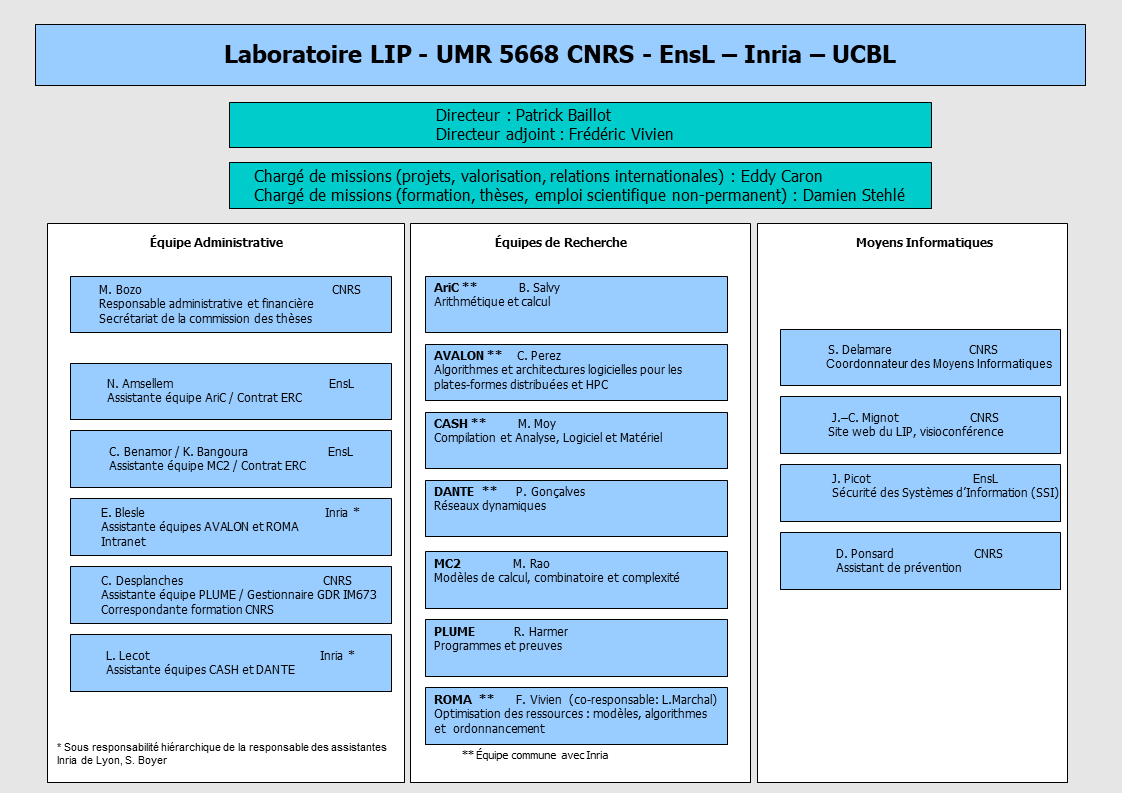
\includegraphics[scale=0.58]{partie1/images/organigramme.png}
	\caption{Organigramme du LIP au 10 Avril 2018 \cite{organigramme}}
\end{figure}
\subsubsection{Des métiers variés}
Le projet du Laboratoire de l'Informatique du Parallélisme est de mettre en relation l'informatique fondamental et sa mise en œuvre pratique dans les institutions. Ainsi le laboratoire crée un lien fort entre informatique et d'autres sciences comme les mathématiques, les sciences du vivant ou, plus globalement, les sciences fondamentales.\cite{presUCBL}\\

Les chercheurs du \gls{lip} possèdent un socle commun : l'algorithmie et l'utilisation efficace des ressources. Ils organisent leurs recherches autour de deux grands axes :
\begin{itemize}
	\item La conception, l'utilisation et l'adéquation aux besoins des applications des futurs architectures de calcul (traitement de données, calcul fondamental) et de communication (réseaux)
	\item L'étude des modèles et des méthodes en informatique : compléxité, algorithmie, développement logiciel et matériel, avancée technologiques etc.\\
\end{itemize}

Ainsi, le laboratoire ne compte pas dans ses rang uniquement des expert de l'informatique. D'autres profils bien différents sont mis en valeurs dans les 7 équipes-projets que nous allons présenter.
\newpage

\textbf{AriC - Arithmetic and Computing}\\
AriC est une grande équipe projet commune avec l'\gls{inria} composée d'une vingtaine de membres. Elle à pour but d'améliorer le calcul, en terme de performance, d'efficacité et de fiabilité. Ses 3 principaux projets de recherche portent sur les sujets suivants :
\begin{itemize}
	\item Les réseaux euclidiens : algorithme et cryptologie,
	\item Les méthodes d'approximation efficaces en calcul formel,
	\item Le calcul fiable à haute performance, avec virgule flottante et précision d'au plus une centaine de bits.
\end{itemize}
Au delà de la recherche cette équipe à une véritable vocation à la diffusion et à la vulgarisation de leurs travaux, ce qui passe par la multiplication des interventions dans les lycées ou autre institutions d'enseignement et la publication d'articles et d'ouvrages \cite{aric}.\\

\textbf{Avalon - Algorithms and Software Architectures for Distributed and HPC Platforms}\\
L'objectif de l'équipe commune \gls{inria} Avalon est de concevoir des modèles de programmations, des systèmes et des algorithmes pour exécuter des applications sur des ressources tout en satisfaisant les contraintes des utilisateurs (e.g.\ coût, performances) et des administrateurs (e.g.\ maximisé l'usage des ressource, minimiser la consommation d'énergie).
L'équipe se concentre en particulier sur le profilage et la modélisation d'applications gourmandes en énergie et en données, la gestion des données et l'ordonnancement des applications sur des architectures de supercalculateurs \cite{avalon}.\\

\textbf{CASH - Compilation and Analyses for Software and Hardware}\\
La vision de l'équipe commune \gls{inria} CASH est d'utiliser l'architecture \gls{dataflow} pour le traitement des données par les supercalculateurs. Son but est d'utiliser les caractéristiques particuliers du matériel informatique afin de fournir des couples matériel-logiciel efficaces énergétiquement au développeur final. Pour ce faire elle travaille sur les axes d'études suivants :
\begin{itemize}
	\item Développer l'architecture \gls{dataflow},
	\item Améliorer les algorithmes de compilation,
	\item Développer la compilation matériel, qui consiste à transformer un programme informatique en un circuit électronique physique,
	\item Émuler les \glspl{systemepuce} pour faciliter leur optimisation \cite{cash}.\\
\end{itemize}

\textbf{DANTE - Dynamic Network}\\
L'objectif principal de l'équipe commune \gls{inria} DANTE est de poser des bases solides à la caractérisation des réseaux dynamiques et des processus dynamiques se produisant sur des réseaux à grande échelle. Afin de développer des outils d'une pertinence pratique en situation réelle, elle fonde ses études méthodologiques sur des jeux de données réelles. Ses 3 grands thèmes de recherche sont :
\begin{itemize}
	\item Le traitement du signal basé sur les graphes,
	\item La théorie des graphes dynamiques,
	\item Les \glspl{algodistrib} pour les réseaux dynamiques \cite{dante}.
\end{itemize}
\newpage
\textbf{MC2 - Models of computation, Complexity, Combinatorics}\\
L'équipe MC2 à pour but de comprendre les possibilités et les limitations des algorithmes efficace. Pour ce faire elle crée et analyse des algorithme jusqu'à leurs limites. Parmi les différents domaines des mathématiques au cœur de ses problématiques, l'équipe MC2 se concentre sur l'algèbre et l'\gls{analysecombinatoire}. Ces deux domaines sont des sources de problèmes algorithmiques qui jouent un rôle clé dans la théorie de la \gls{complexite} \cite{mc2}.\\

\textbf{PLUME - Programs and Proof}\\
Les recherches menées par l'équipe PLUME s'articulent autour de deux thèmes fortement imbriqués : les fondements logiques des langages de programmation et la théorie des systèmes informatiques. Elle met au centre de ses recherche la logique mathématique afin de trouver comment écrire des programmes sûrs ou comment vérifier formellement des systèmes informatique complexes \cite{plume}.\\

\textbf{ROMA - Resource Optimization : Models, Algorithms and Scheduling}\\
L'équipe commune \gls{inria} ROMA vise à concevoir des modèles, des algorithmes et des stratégies d'ordonnancement pour optimiser l'exécution d'applications scientifiques sur des supercalculateurs. Plus spécifiquement, ROMA vise à obtenir la "meilleure" performance possible du point de vue de l'utilisateur (e.g.\ le temps d'exécution de l'application) tout en utilisant les ressources aussi efficacement que possible \cite{roma}.\\

Ainsi, le Laboratoire de l'Informatique du Parallélisme possède un impressionnant savoir faire dans de nombreux domaines de l'informatique et produit de nombreuses ressources pour des institutions publiques et privés, comme nous allons le voir.

\subsubsection{Une production conséquente}
Le Laboratoire de l'Informatique du Parallélisme est plutôt prolifique dans la quantité de production. Depuis 2000, 2502 publications ont été publiés et sont disponibles sur des plateforme en ligne comme les archives ouvertes HAL. En effet le laboratoire est dans une véritable démarche de production de connaissances, mais cela ne l'empêche pas de s'autofinancer grâce à des contrats industriels et des projets institutionnels régionaux, nationaux et internationaux \cite{reportHCERES}. 2 brevets ont même été déposés.\\

Le laboratoire encourage également les ambitions d'entrepreneuriat de ses membres avec la création de 5 start-ups dans le domaine du numérique depuis 2010 \cite{presUCBL}.\\

Enfin, les différentes équipes du laboratoire produisent également de nombreuses ressources logicielles open-source à destinations des institutions, les industriels et même des particuliers que l'on peut retrouver sur les plateforme de partage de code source en ligne.
\subsection{L'équipe Avalon en détails}
L'équipe dont je fais parti durant ce stage est l'équipe Avalon. Cette équipe créée le 1er Février 2012 \cite{avalonAR2012} est une équipe-projet du Laboratoire de l'Informatique du Parallélisme commune à l'\gls{inria} et composée de 22 membres : 8 universitaires permanents, 2 universitaires temporaires, 4 membres permanents et 8 doctorants. Elle est située au troisième étage de l'aile sud du bâtiment M7 sur le site Monod de l'École Normale Supérieure de Lyon.

\subsubsection{Les membres de l'équipe}
Parmi les 22 membres de l'équipe, voici un rapide aperçu de ceux que j'ai côtoyé durant mon stage :\\

\textbf{Universitaires permanents}
\begin{figure}[h!]
   \begin{minipage}{0.33\textwidth}
		\centering
		
\includegraphics[height=3cm]{partie1/images/christian.jpg}\\
		\textbf{Christian Perez}\\
		Chef de l'équipe\\Chercheur sénior Inria
	\end{minipage}\hfill
	\begin{minipage}{0.33\textwidth}
		\centering
		
\includegraphics[width=3cm]{partie1/images/eddy.jpeg}\\
		\textbf{Eddy Carron}\\
		Responsable administratif\\Enseignant chercheur
	\end{minipage}\hfill
	\begin{minipage}{0.33\textwidth}
		\centering
		
\includegraphics[width=3cm]{partie1/images/laurent.jpg}\\
		\textbf{Laurent Lefèvre}\\
		Mon maître de stage\\Chercheur Inria
	\end{minipage}
\end{figure}

\textbf{Universitaires temporaires}
\begin{figure}[h!]
	\begin{minipage}{0.48\textwidth}
		\centering
		
\includegraphics[height=3cm]{partie1/images/marco.jpg}\\
		\textbf{Marcos Dias de Assuncao}\\
		Chercheur
	\end{minipage}\hfill
	\begin{minipage}{0.48\textwidth}
		\centering
		
\includegraphics[height=3cm]{partie1/images/cyril.jpg}\\
		\textbf{Cyril Seguin}\\
		Chercheur PostDoc\\Expert Cloud et Sécurité
	\end{minipage}\hfill
\end{figure}

\textbf{Équipe}
\begin{figure}[h!]
	\begin{minipage}{0.33\textwidth}
		\centering
		
\includegraphics[height=3cm]{partie1/images/evelyne.jpeg}\\
		\textbf{Evelyne Blesle}\\
		Assistante administrative
	\end{minipage}\hfill
	\begin{minipage}{0.33\textwidth}
		\centering
		
\includegraphics[width=3cm]{partie1/images/simon.jpeg}\\
		\textbf{Simon Delamare}\\
		Ingénieur de recherche
	\end{minipage}\hfill
	\begin{minipage}{0.33\textwidth}
		\centering
		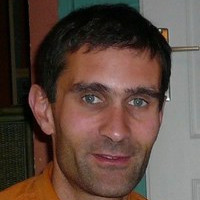
\includegraphics[width=3cm]{partie1/images/matthieu.jpeg}\\
		\textbf{Matthieu Imbert}\\
		Ingénieur de recherche
	\end{minipage}
\end{figure}
\newpage
\textbf{Doctorants}
\begin{figure}[h!]
	\begin{minipage}{0.33\textwidth}
		\centering
		
\includegraphics[height=3cm]{partie1/images/issam.jpeg}\\
		\textbf{Issam Raïs}\\
		Thèse sur l'étude de la consommation énergétique des supercalculateurs
	\end{minipage}\hfill
	\begin{minipage}{0.33\textwidth}
		\centering
		
\includegraphics[width=3cm]{partie1/images/dorra.png}\\
		\textbf{Dorra Boughzala}\\
		Thèse sur la simulation de la consommation d'énergie des architecture hétérogènes
	\end{minipage}\hfill
	\begin{minipage}{0.33\textwidth}
		\centering
		
\includegraphics[width=3cm]{partie1/images/alexandre.jpg}\\
		\textbf{Alexandre da Silva Veith}\\
		Thèse sur les algorithmes pour l'analyse des flux élastiques du Big-Data
	\end{minipage}
\end{figure}
\begin{figure}[h!]
	\begin{minipage}{0.33\textwidth}
		\centering
		
\includegraphics[height=3cm]{partie1/images/hadrien.jpeg}\\
		\textbf{Hadrien Croubois}\\
		Spécialisé dans les processus parallèles et les systèmes distribués
	\end{minipage}\hfill
	\begin{minipage}{0.33\textwidth}
		\centering
		
\includegraphics[width=3cm]{partie1/images/felipe.jpg}\\
		\textbf{Felipe Rodrigo de Souza}\\
		Thèse sur les algorithmes de provisionnement des réseaux
	\end{minipage}\hfill
	\begin{minipage}{0.33\textwidth}
		\centering
		
\includegraphics[width=3cm]{partie1/images/valentin.jpg}\\
		\textbf{Valentin Lorentz}\\
		Thèse sur la traçabilité énergétique des données
	\end{minipage}
\end{figure}

\subsubsection{Le contexte de création}
Formée le 1 Février 2012, l'équipe Avalon est une véritable réponse aux changements effrénés de l'informatique.
L'évolution très rapide du matériel informatique en terme de communication, de traitement de données et de virtualisation a fait émerger des nouveaux besoins pour l'utilisateur. En effet la complexité des systèmes informatiques augmente !
Il existe aujourd'hui de nombreuses variétés de plateformes à grande échelle disponibles pour des chercheurs ou des industriels qui souhaitent satisfaire leurs besoins en traitement de données : agrégation de \glspl{cluster}, grand \glspl{datacenter}, supercalculateurs etc.
Chacune de ces plateformes dispose de spécificités intrinsèques, d'accès et d'utilisation qui ont un impact important sur l'architecture et l'exécution des applications qui souhaitent les utiliser.
Elles intègrent de nombreuses fonctionnalités obligatoires comme le sécurité, la virtualisation, le \gls{load-balancing} ou autres qui augmentent encore plus leur complexité d'utilisation.
C'est dans ce contexte que l'équipe Avalon a été créée, la réponse qu'elle apporte est d'aller plus loin dans l'abstraction de ces plateformes pour assurer à l'utilisateur une utilisation simplifiée tout en gardant l'ensemble des fonctionnalités disponibles. \cite{avalonAR2012}

\subsubsection{La vision de l'équipe}
La vision de l'équipe Avalon est de considérer l'ensemble du système, de la ressource à l'application, afin de concevoir des outils simples à utiliser par les programmeurs tout en permettant une exploitation efficace des ressources.
L'équipe se concentre en particulier sur la gestion de l'élasticité (i.e\ la capacité à s'adapter aux besoins des applications le plus rapidement possible) des plateforme parallèles et distribués ainsi que leur efficacité énergétique. \cite{avalonAR2012}\\

L'équipe souhaite pouvoir mettre à disposition d'autres équipes de recherche travaillant dans d'autres sciences des ressources informatiques à haute performance de manière simple à utiliser.

Voici quelques exemples de disciplines qui pourrait avoir recours aux travaux de l'équipe Avalon :
\begin{itemize}
	\item La biologie, avec par exemple le séquençage de l'ADN,
	\item L'étude du climat, qui demande une quantité de paramètres impressionnante pour simuler les changements de climat prochains,
	\item L'astrophysique, qui est demandeuse de simulations pour comprendre les phénomènes physique qui nous entoure, la formation des galaxies, pour étudier la matière noire etc.
\end{itemize}
\subsection{Mon environement au sein du laboratoire}
Dans cette partie nous allons voir dans quel environement de travail j'ai évolué tout au long de mon stage au sein du laboratoire. Nous présenterons tout d'abord comment s'est organisé le travail, ensuite dans quel environement technique j'ai évolué et enfin quelles sont mes interactions avec les autres membres de l'équipe.

\subsubsection{Les horaires de travail}
Le travail au laboratoire est assez librement organisé. En effet, pendant toute ma période de stage j'ai eu, dans la limite d'effectuer 35 heures par semaines, des horaires libres. Cela m'a permis d'organiser facilement d'autres tâches importantes de cette période, notamment les entretiens avec les écoles d'ingénieurs pour mon admission en alternance, le forum d'entreprise obligatoire de Polytech ou encore mes entretiens individuels avec des entreprises dans le but de dénicher un contrat d'apprentissage.\\

Contrairement à lorsque j'étudiais à l'IUT où j'aurais farouchement défendu ma pause de midi de 2h ainsi que mes pauses de 20 minutes toutes les deux heures, je n'ai pas spécialement ressenti pendant ce stage le besoin de prendre de longues pauses. C'est pour cela, qu'après quelques jours, je me suis basé sur un rythme de travail de 9h--16h30.\\

Arriver à 9h est déjà une grande différence par rapport à l'IUT, c'est tout d'abord une heure plus tard, mais mon temps de trajet étant également plus court pour aller au laboratoire que pour aller à l'IUT, cela me permet de me lever 1h20 plus tard tous les matins.\\

Pour le temps de midi, une petite particularité du laboratoire est qu'il utilise pour manger le restaurant universitaire de l'ENS Lyon, ainsi pour ne pas faire la queue, les équipes ont décidés de descendre manger à 11h30. Tous les midis une partie de l'équipe Avalon descend ensemble manger pendent environs 30 minutes, puis remonte. Il reste alors 4h30 de travail pour arriver aux 7 heures de travail quotidien.\\

Je me suis fais la réflexion que ce rythme de travail n'est peut-être pas le plus adéquat en raison de son déséquilibre entre le temps de travail du matin et de l'après midi. Mais je n'étais pas convaincu par le fait d'arriver à 8h et de repartir à 15h30.
 
\subsubsection{Les locaux}
Ce stage s'est déroulé dans les locaux du LIP, au troisième étage du bâtiment M7 du site Monod de l'ENS Lyon. Pratiquement tous les membres de l'équipe Avalon sont situés au même endroit : un grand couloir dessert de part et d'autres des bureaux de deux, parfois trois, personnes.\\

Au début de mon stage j'étais situé dans le dernier bureau du couloir que je partageais avec \textbf{Issam Raïs}, doctorant sous la supervision de mon maître de stage Laurent Lefèvre. Le 22 mai, une réorganisation des bureaux a été faites, j'ai quitté Issam pour rejoindre, dans le bureau situé juste avant, \textbf{Lucas Besnard}, un camarade de promotion qui effectue également son stage au LIP, mais qui ne travaille pas sur le même sujet que moi.\\

Les bureaux sont relativement spacieux, possèdent une armoire commune ainsi qu'un casier individuel. Le principale problème est que l'équipe est situé dans l'aile Sud du bâtiment et que les bureaux sont équipés d'une grande baie vitré coté Sud. Lorsqu'il y a du soleil le travail devient très vite difficile en raison des températures. Heureusement nous avions la possibilité de nous réfugier dans la bibliothèque de l'ENS, qui est climatisée, si cela devenait intenable.\\

Le bâtiment possède également des boxs de travail ou nous pouvions nous retrouver pour travailler à plusieurs, ainsi qu'une grande salle de réunion. Après le couloir, un solarium était également à notre disposition avec des transats, qui m'ont bien été utiles lors de la lecture de publications scientifiques.

\subsubsection{L'environement matériel}
Le laboratoire pouvait me fournir un ordinateur portable ainsi qu'une station d'accueil pour effectuer me travaux. Cependant ces machines n'étant pas très performantes on m'a conseillé d'utiliser mon ordinateur personnel.\\

On m'a par contre fourni un deuxième écran, qui est quelque-chose que je trouve de plus en plus indispensable. Il est d'ailleurs tombé en panne quelques semaines plus tard, probablement à cause de la chaleur, mais Issam m'a très gentiment prêté un de ses écrans qu'il n'utilisait pas.

\subsubsection{L'environement technologique}
L'équipe Avalon ne possède pas vraiment d'environement technologique propre, car chaque membre utilise les technologies les plus pertinentes pour chaque tâche. Cependant, elle utilise activement le plateforme \emph{Grid'5000} que je vais présenter.\\

\begin{figure}[h!]
	\centering
	
\includegraphics[width=5.5cm]{partie1/images/grid5000_logo.png}
	\caption{Logo de la plateforme Grid'5000}
\end{figure}

Grid'5000 est un banc d'essai à grand échelle pour la recherche expérimentale en informatique. Cette plateforme met à disposition des chercheurs un très grande quantité de ressources informatiques : plus de 1000 serveurs, 8000 cœurs de processeur regroupés en \glspl{cluster}. Elle est utilisé par une communauté de plus de 500 utilisateurs et est hébergée sur une dizaine de sites en France. \cite{grid5000home}\\

Elle est à la pointe de la technologie avec notamment une connexion au réseau de 10Gbit/s (5000 fois meilleure que la box qui vous connecte à Internet), des connectiques \emph{Infiniband} qui permettent un débit jusqu'à 56Gbits/s ou encore les processeurs ultra performants \emph{Xeon PHI} du constructeur leader \emph{Intel}.\\

La plateforme intègre de nombreux outils de monitoring et de mesure afin de permettre des expérimentations et leurs interprétations très précises. Elle possède notamment un arsenal de Wattmètres qui mesurent au plus près de la machine la consommation du matériel et qui sont beaucoup utilisés par les membres de l'équipe Avalon, notamment par Issam et Dorra pour leurs thèses et mon camarade Lucas pour son stage.\\

Afin de nous former, Lucas et moi, à l'utilisation de cette plateforme nous avons été formé par \textbf{Dorra Boughzala}, qui venait d'effectuer une formation complète. Nous avons passé 2 à 4 heures par jour en sa compagnie pendant la première semaine de notre stage. Je n'avais jamais utilisé une telle plateforme, mais étant déjà familiarisé aux environnements Linux ainsi qu'à certains concepts, j'ai pû assez facilement m'approprier l'outils, qui s'avère extrêmement intéressant et puissant.
 
\subsubsection{L'environement humain}
Évidemment, un laboratoire de recherche est international, un certain nombre des membres de l'équipe ne sont donc pas français. Tout le monde parle bien l'anglais ce qui permet de très bien se comprendre, mais la barrière de la langue se fait parfois ressentir lorsqu'on troque les interactions formelles pour des interactions plus amicales. Les interactions avec les différents membres de l'équipe et du laboratoire sont d'ailleurs très décontractés, tout le monde se tutoie, par exemple.\\

Pour ma mission je ne communiquais qu'avec Laurent, mon maître de stage qui prennait note de l'avancement du projet tout en m'aiguillait et en me proposant des pistes à suivre, parfois en me fournissant des publications scientifiques. Il n'a cependant pas participé à la phase de développement, où j'étais en toute autonomie.

\subsubsection{Les groupes de travail}
Lorsque l'équipe en ressent le besoin, des groupes de travail sont organisés. Toute l'équipe se retrouve ensemble dans une sale de réunion. Souvent elle procède à une \emph{round table}, qui consiste à présenter ce sur quoi on travaille, ce que l'on a fait depuis la dernière \emph{round table} et ce que l'on a prévu de faire pour la suite. Mais parfois il peut s'agir d'un membre de l'équipe qui souhaite présenter, une technologie, son travail ou tout autre chose.\\
Les membres mettent également par écrit ce qu'ils ont dit durant le groupe de travail, ce qui permet à Alexandre de mettre à jour le site internet de l'équipe Avalon.
\newpage
\section{La mission du stage}
\emph{TODO: Rédiger l'introduction de la partie}

\subsection{Présentation de la mission}
Ma mission pendant ce stage est de créer un simulateur informatique d'empreinte environnementale des centres de données. Nous allons présenter dans cette partie, en quoi cette mission s'intègre dans des problématique contemporaines et comment nous allons faire pour y répondre.

\subsubsection{Le contexte}
Face à la constante augmentation des besoins en ressources informatiques, que ce soit de calcul, de stockage ou de communication, ainsi que l'augmentation de leur qualité (disponibilité, rapidité etc.) de nombreux centre de données doivent être construits pour répondre à ces besoins. L'échelle de grandeur de ces centres de données doit être à l'échelle du besoin, ainsi ils sont de plus en plus imposants et construits de plus en plus proche des environements urbains qui concentrent les usages.\\

Cela n'est pas sans conséquences, les centres de données génèrent une très grosse empreinte environnementale. Leur consommation d'énergie est record, pouvant aller jusqu'à plus de 20GW, en effet l'informatique est très gourmand en énergie et nécessite d'être refroidi par des systèmes encore plus gourmands. Ils ont un très gros impact sur le territoire : grosse surface au sol occupée, génèrent de la chaleur, du bruit et des vibrations qui peuvent gêner le voisinage. Ils possèdent des groupes électrogènes de secours, qui apportent des risques supplémentaires notamment par le stockage de grande quantités de fioul et impactent le voisinages via leur tests réguliers qui génèrent une grande quantité de fumée.\\

Une illustration de ce nouveau besoin en ressources informatiques au plus près des villes sont les jeux olympique 2024 à Paris. En effet, le trafic de données sur la région parisienne va grandement augmenter, de part les besoins des institutions sportives, mais également par ceux des spectateurs qui sont aujourd'hui tous connectés à internet par leur smartphone. Il va donc falloir intégrer dans le territoire de nouveaux centres de données pour traiter ces nouvelles données. Il serait donc intéressant de fournir aux urbanistes et aux architectes un outils qui permettrait de comparer les projets de centre de données entre eux et de mesure leur impact sur l'environnement.\\

Ainsi, l'Institut d'aménagement et d'urbanisme de la région Île-de-France et l'Ecole d'architecture de la ville et des territoires, acteurs de l'urbanisme en région parisienne, se sont associés avec le Laboratoire de l'Informatique du Parallélisme, qui n'a plus à prouver son expertise sur les sujets environnementaux en lien avec l'informatique, afin de s'entraider dans la réflexion de nouveaux projets de centre de données en environement urbain.

\subsubsection{Les enjeux}
Les travers des centres de données ne sont pas ignorés par les industriels et les institutions. Les pratiques de \emph{GreenIT}, littéralement \emph{informatique vert}, se développent de plus en plus. Le réchauffement climatique est un enjeu planétaire, et la réduction des émissions de gaz a effet de serre peut se faire via la diminution de la consommation d'énergie des centres de données qui représentait déjà, en France, 4\% de la production d'électricité en 2015 \cite{percentageElectricite}. Les industriels, eux ont tout de suite vu que la réduction de la consommation d'énergie implique obligatoirement la diminution des coûts. De plus ayant remarqué l'attrait du public et des institutions pour l'efficacité énergétique de leurs centres de données, ils peuvent rentabiliser leurs actions en faveur de l'efficacité énergétique par des campagnes de green-washing.

La population elle aussi devient méfiante à l'égard des nouveaux projets de centre de données et pointent les nuisances, parfois illégales, qu'ils génèrent sur le voisinage, jusqu'à porter plainte \cite{plainte}, ce qui porte préjudice aux société exploitantes.\\

Les porteurs de projets, quant-à-eux ne possèdent pas toujours des outils simples qui permettent de mesurer l'impact de leur projet sur l'environement. Ils ne possèdent d'ailleurs pas toujours des connaissances en informatique, il est donc primordiale d'apporter un outils simple, compréhensible par tous, fiable et assez puissant pour prendre en compte toutes les caractéristiques des centres de données afin de les aider dans la construction de leur projet.

\subsubsection{L'outils demandé}
Pour répondre à ces besoins, nous avons imaginé un outils informatique permettant de simuler l'impact environnementale d'un centre de données. Cet outils devra tout d'abord être facilement compréhensible par un architecte ou un urbaniste car ils seront probablement les utilisateurs finaux. Le simulateur devra prendre en compte une multitude de paramètres, décrivant un centre de données, entrés par l'utilisateur, les compiler et les présenter à l'utilisateur sous une forme permettant des les analyser. Pour ce faire, nous utiliserons un certain nombre d'indicateur de \emph{Green IT} reconnus par des institutions ou des organismes et les présenterons à l'utilisateur via un rapport détaillé généré automatiquement par l'outils.\\

Le simulateur devra être construit autour de trois grands blocs : le matériel informatique, le refroidissement, et les sources d'énergie électrique. L'utilisateur doit pouvoir entrer la liste du matériel informatique du centre de données, ce qui permettra de calculer la chaleur générée ainsi que la consommation d'énergie. Ensuite, il devra pouvoir choisir les paramètres du refroidissement afin de traiter la chaleur générée, ce qui fera augmenter la quantité d'électricité consommée par le site. Enfin il devra pouvoir choisir comment le centre de données est alimenté électriquement pour répondre à ses besoins énergétiques.\\

Au début du projet nous souhaitions un outils fonctionnel et puissant mais pas nécessairement beau ou très ergonomique, nous verrons par la suite que j'ai volontairement modifié cette direction afin de donner à l'utilisateur une meilleur expérience.
\subsection{La recherche bibliographique}

\subsection{La développement}
Une fois la recherche bibliographique à peu près terminé, nous avons une idée plus clair de à quoi le simulateur devrait ressembler. Nous présenterons dans cette partie les différentes tâches effectués lors du développement du simulateur.
\emph{TODO: GANT}

\subsubsection{Le choix des outils}
Pour le développement de ce simulateur j'ai décidé d'utiliser le langage \gls{java}. En effet, j'avais déjà une expérience sur ce langage qui à été consolidé par l'enseignement reçu en DUT. \gls{java} est également plateforme ce qui permet au simulateur de pouvoir fonctionner sous la plupart des systèmes d'exploitation.\\

Pour ma gestion des librairies j'ai utilisé la technologie \gls{maven} qui permet de gérer très facilement ses librairies ainsi que la compilation des projets Java. Même si il peut y a voir quelques fois des complications, cet outils est généralement très facile d'utilisation.\\

J'ai décidé d'utiliser pour l'interface utilisateur la technologie \gls{javafx} qui est désormais intégré dans l'installation par défaut de Java. J'avais découvert cette technologie via mes camarades de promotions et l'est utilisé pour la première fois dans le projet de groupe du cours de \emph{CPOA} où nous avions réaliser une application de gestion d'un tournois de tennis. Le choix de cette technologie est logique au vu de sa puissance et sa facilité d'utilisation en comparaison des technologies plus anciennes comme \emph{AWT} ou \emph{Swing}.\\
Cependant, je n'étais pas totalement satisfait du rendu graphique de JavaFX, c'est pour cela que j'ai cherché une alternative qui me permette d'embellir mes interface graphiques. C'est alors que j'ai découvert la librairie \emph{JFoenix} qui implémente le Matérial Design, qui est un courant de design graphique numérique initié par Google, en JavaFX.

\subsubsection{L'architecture générale}
Avant de développer chaque fonctionnalité du simulateur il faut tout d'abord réfléchir à comment va s'organiser le code source. Le simulateur va prendre la forme d'une succession d'écrans dans lesquelles l'utilisateur pourra saisir des valeurs, une fois les valeurs vérifiés, l'utilisateur pourra passer à l'écran suivant. Une fois qu'un écran est complété, l'utilisateur peut revenir en arrière sur un autre écran afin de modifier ses valeurs.\\

Pour arriver à ce résultat, j'ai mis en pratique une notion que nous avons appris en DUT : le modèle MVC.
\begin{figure}[h]
	\begin{center}
		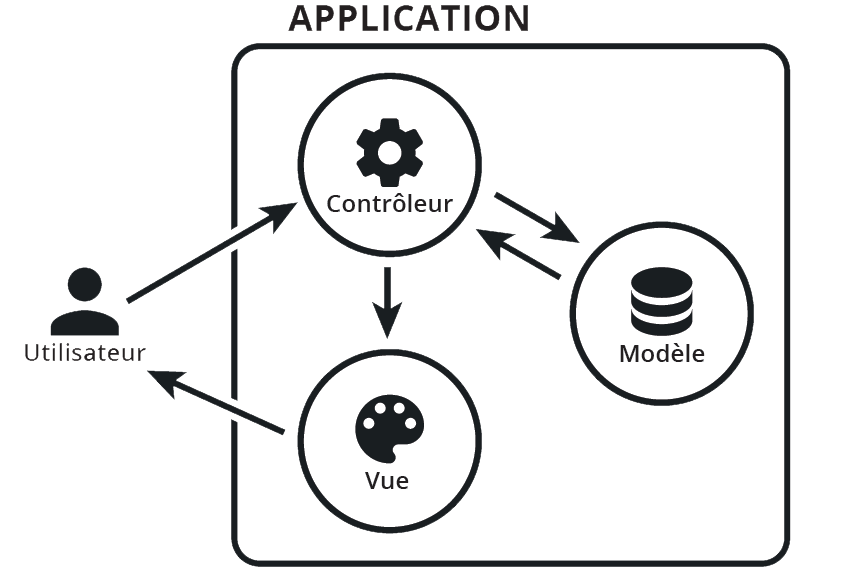
\includegraphics[scale=0.70]{partie2/images/mvc.png}
		\caption{Schéma du modèle MVC}
	\end{center}
\end{figure}

Le modèle MVC (Modèle-vue-contrôleur) est un modèle d'architecture logiciel destiné aux interfaces graphiques. Il se découpe en 3 modules effectuant chacun une action spécifique :
\begin{itemize}
	\item Le modèle qui s'occupe de récupérer les données à afficher dynamiquement,
	\item La vue qui contient toutes les composants graphiques,
	\item Le contrôleur qui s'occupe de récupérer et traiter les actions faites par l'utilisateur.\\
\end{itemize}

Ainsi chaque écran possède une vue et un contrôleur qui parfois va chercher des information dans un modèle. La vue est stocké sous forme de fichier FXML, qui est une implémentation du langage de balisage XML propre à JavaFX et qui nous permet de construire des vue à la manière d'une page web. Chaque vue, en plus des éléments graphiques, possède un nom, un numéro d'apparition ainsi qu'une référence vers leur contrôleur associé.
Afin de charger toutes les vues en mémoire le plus facilement possible, on les stocke dans un même dossier, ainsi au lancement du simulateur il suffira de récupérer la liste des fichiers de ce dossier, de lire le FXML de chaque fichier afin de créer la vue et d'y associer le contrôleur associé grâce à la référence stockée dans le fichier.

\subsubsection{L'architecture des contrôleurs}
Pour que le simulateur soit fonctionnel j'ai besoin d'effectuer certaines actions à certains moments dans l'exécution du programme. Je dois par exemple initialiser les composants graphiques de la vue une seule fois au tout début du programme pour qu'ils soient fonctionnel. J'ai également besoin, parfois d'effectuer des actions à chaque fois que l'utilisateur va sur un écran. Je dois également pouvoir être capable de changer les lignes de textes lorsque l'utilisateur demande à changer de langue.\\
Pour ce faire j'ai créé un \emph{interface} Java appelé \code{ViewController}, il s'agit d'une sorte de modèle que je peux appliquer à mes contrôleur afin qu'ils implémentent les modules que j'ai définis dans l'interface. Cet interface comporte donc 3 modules :
\begin{itemize}
	\item L'initialisation, qui s'exécute une seule fois par exécution du simulateur, au chargement de la vue en mémoire,
	\item Le chargement, qui s'exécute à chaque fois que l'utilisateur change d'écran,
	\item L'application de la langue, qui s'exécute à lorsque l'utilisateur souhaite changer la langue.
\end{itemize}
Ces trois modules étant essentiels pour chaque écran, tous mes contrôleur de vue implémentent cet interface.\\

J'ai également créé un autre interface Java, appelé \code{FormViewController}, qui lui ne sera appliqué qu'aux vues qui comporte un formulaire car il permet en implémentant les 3 modules suivant de gérer les champs des formulaire :
\begin{itemize}
	\item La sauvegarde, qui vérifie si les champs sont valides et lance la sauvegarde
	\item Le remplissage des champs, qui s'exécute lorsque l'on charge un sauvegarde en entrant les valeurs lues
	\item Le nettoyage des champs, qui supprime toutes les valeurs contenus dans les champs
\end{itemize} 

\subsubsection{La notion de simulation}
Pour que l'utilisateur puisse gérer facilement ses différentes configuration de centre de données qu'il rentre dans le simulateur j'ai décidé d'avancer la notion de simulation. Une simulation est tout simplement une instance du simulateur, elle contient un nom, des auteurs ainsi que tous les paramètres entrés par l'utilisateur durant l'exécution du programme. Cette simulation peut être facilement stocké et lue depuis le disque dur de l'utilisateur.\\

D'un point de vue technique, la simulation représente un objet Java que nous sérialisons au format JSON afin de la stocker sur le disque. Il nous suffira ensuite de la dé-sérialiser pour la charger en mémoire. J'ai fais le choix du format JSON car il est facilement lisible par l'humain et qu'il est extrêmement utilisé par les développeurs, la plupart des langages proposent des librairie pour le lire. Ainsi les fichiers de sauvegarde du simulateur pourrons facilement être utilisé dans d'autres programmes, même si ils ne sont pas développés en Java.

\subsubsection{La gestion de la langue}
Le laboratoire étant international j'ai naturellement penser à implémenter la possibilité de changer la langue du simulateur. Pour ce faire chaque ligne de texte qui est affichée à l'écran est codé par un identifiant unique. Par exemple l'identifiant \code{OPEN\_SIMULATION} représente la phrase \og Ouvrir une simulation \fg{} en français et la phrase \og Open a simulation \fg{} en anglais. Toutes les lignes de textes sont ainsi associé à leur identifiant dans un fichier de langue (que l'on appelle locale) situé dans un dossier de ressource. Chaque fichier contient également le nom de la langue, il nous suffit alors, comme pour les vue, de charger tous les fichiers du dossier afin de récupérer toutes les langues. Pour rajouter une langue au simulateur il faut donc simplement glisser dans le bon dossier un nouveau fichier de langue, sans avoir besoin de modifier le code source.

\begin{figure}[h]
	\begin{center}
		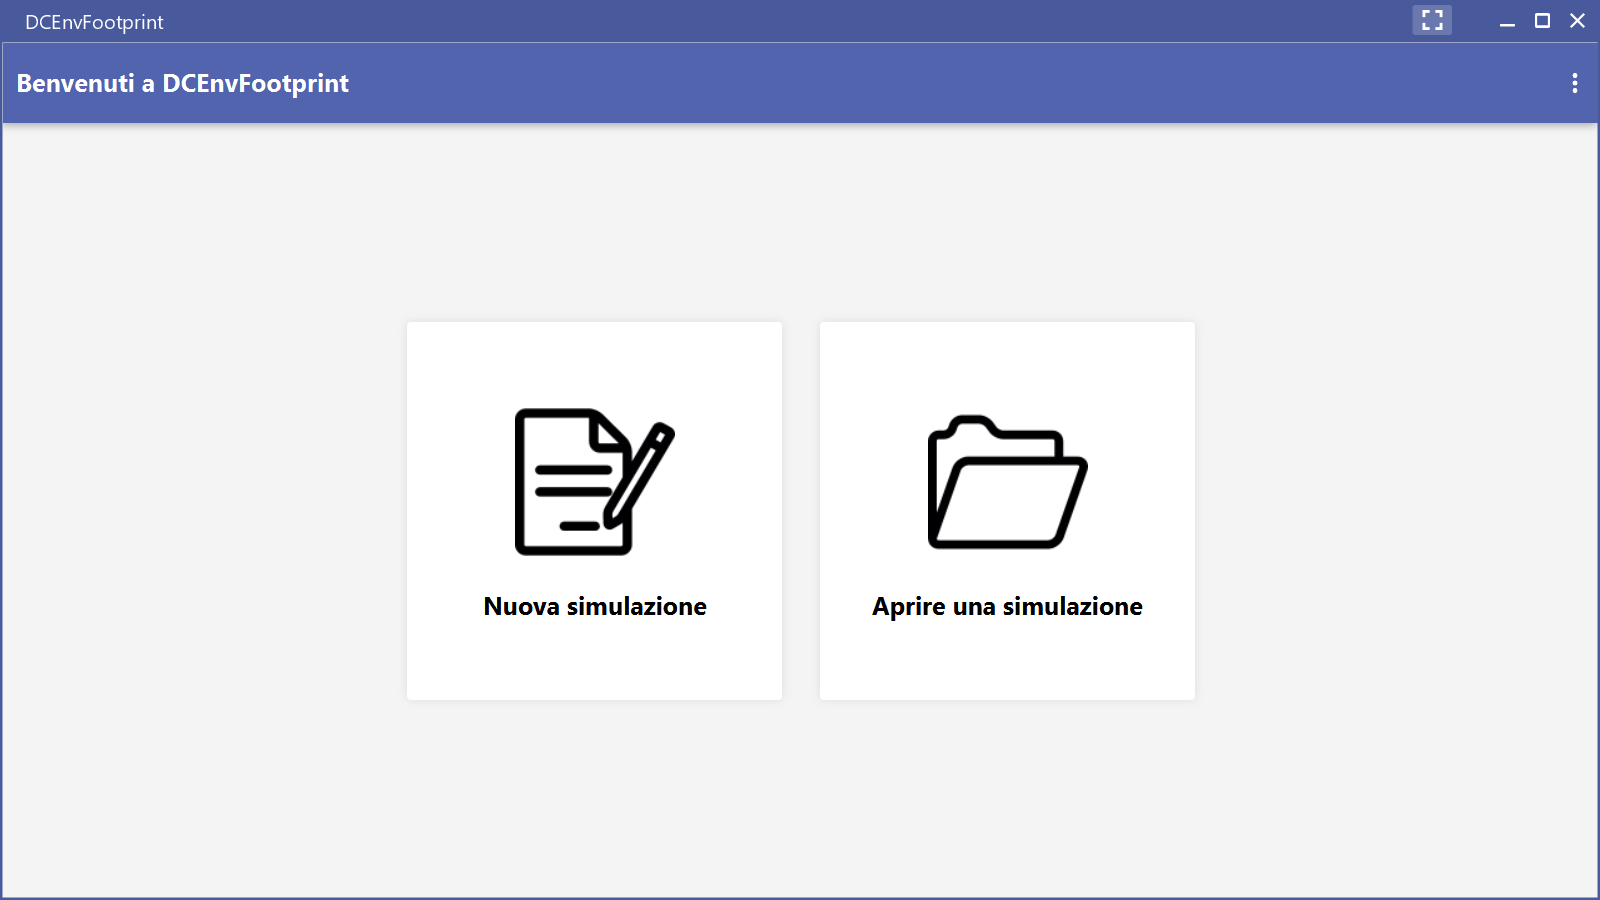
\includegraphics[scale=0.50]{partie2/images/italien.png}
		\caption{Le simulateur réglé en italien}
	\end{center}
\end{figure}
Le choix de la langue de l'utilisateur, qui se fait dans un menu en haut à droite, est sauvegardé. Pour ce faire nous utilisons un fonctionnalité de Java : les \code{Preferences}, qui permettent de stocker des couples clefs-valeurs très facilement sans se soucier du système d'exploitation. Ainsi lorsque l'utilisateur ferme et ré-ouvre le simulateur, la langue est reste inchangée.

\subsubsection{La réflexion autour de l'ergonomie}
Comme l'interaction avec les utilisateurs finaux à été quasiment inexistence, j'ai du pousser un peu plus loin la réflexion sur l'ergonomie que sur un projet plus classique où les retours réguliers des utilisateurs auraient permis de l'affiner. Le simulateur possède donc 2 menus, un menu latéral sur la gauche qui rappelle le nom de la simulation et affiche toutes les étapes de successives que l'utilisateur va suivre. L'utilisateur peut revenir à une étape qu'il a passé, mais ne peux pas aller sur les étapes grisés qui représente celles qu'il n'a pas encore remplis. J'ai également disposé un deuxième menu dans le coin supérieur droit qui permet d'effectuer des actions simples comme créer une nouvelle simulation, en ouvrir une existante, sauvegarde la simulation courante, changer les paramètres de  langues, afficher des informations générales sur le simulateur et quitter l'application.

\begin{figure}[h]
	\begin{center}
		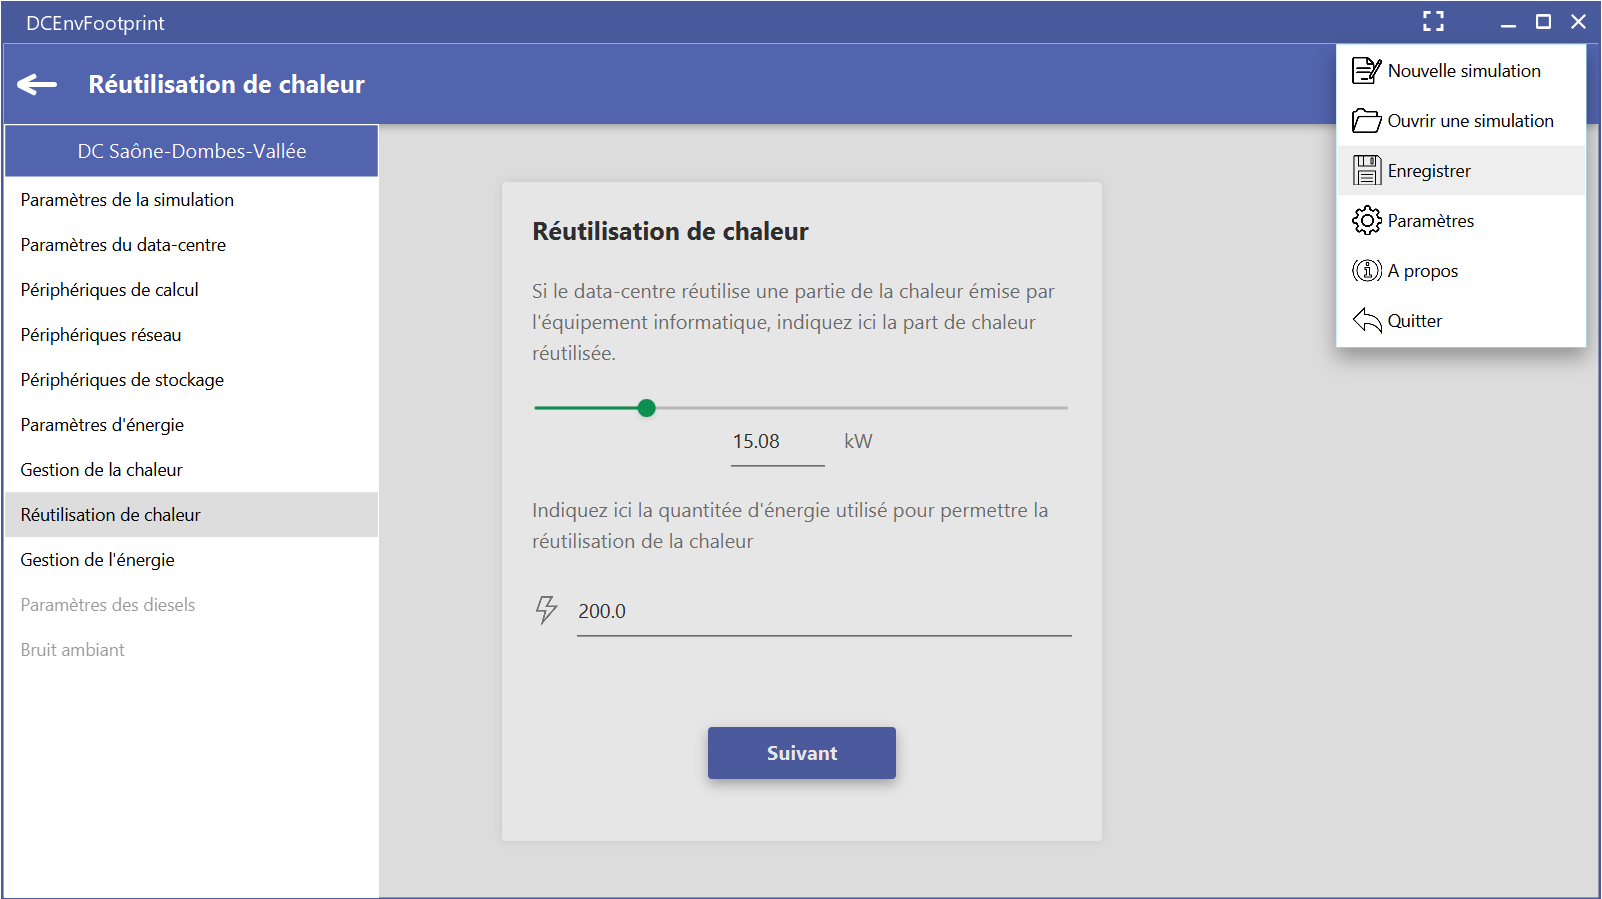
\includegraphics[scale=0.40]{partie2/images/ergonomie1.png}
		\caption{Les menus du simulateur}
	\end{center}
\end{figure}

Comme on peut le voir dans cet exemple, j'ai également fait le choix d'utiliser des composant d'interface graphique facile d'utilisation comme le slider tout en laissant à l'utilisateur le choix de précision avec un champs de texte qui est mis à jour et qui met à jour la valeur du slider. J'en ai utilisé d'autres comme les cartes ou les spinners que vous pourrez apercevoir par la suite.

\subsubsection{Les éléments d'interface personnalisés}
\begin{figure}[h!]
	\begin{minipage}{0.48\textwidth}
		\centering
		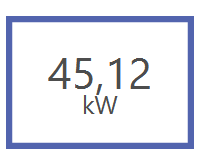
\includegraphics[height=4cm]{partie2/images/customcontrol1.png}
		\caption{Un indicateur de valeur avec unité}
	\end{minipage}\hfill
	\begin{minipage}{0.48\textwidth}
		\centering
		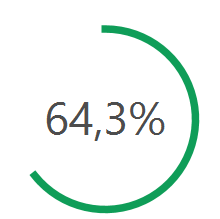
\includegraphics[height=4cm]{partie2/images/customcontrol2.png}
		\caption{Un indicateur de pourcentage}
	\end{minipage}\hfill
\end{figure}

Afin de coller au mieux a ce que j'imaginais pour l'affichage de certains indicateur, j'ai dû personnaliser certains éléments d'interface. J'ai réécris des partie du code source d'éléments graphiques déjà implémenté dans JavaFX ou dans JFoenix et je les ai modifié pour que je puisse les utiliser par la suite. Ainsi j'ai créé un indicateur de valeur avec une unité personnalisable, qui affiche automatique le bon ordre de grandeur de la valeur stocké : si 1000 W sont stocké  l'indicateur affichera 1 kW. J'ai également créé cette afficheur de pourcentage qui est basé sur un élément graphique représentant un temps de chargement.

\subsubsection{La gestion des bases de données}
Pour certaines fonctionnalités le simulateur à besoins d'informations issues de base de données. C'est notamment le cas pour récupérer le poste électrique le plus proche dans le calcul de l'Indice d'Efficacité du Transport Electrique ou pour récupérer l'efficacité énergétique du matériel depuis la base de données \emph{SPEC}.\\
Ces données sont le plus souvent stockés dans des structures de données facilement lisible par l'humain, mais qui ne sont pas très performant pour leur exploitation automatique par un algorithme, comme par exemple les classeurs Excel. Pourtant le simulateur à besoin de faire des requêtes sur ces données pour extraire ce dont il a besoin.\\

Quoi de mieux pour faire des requêtes que d'utiliser le langage SQL que nous avons appris à l'IUT ? Afin d'exploiter les bases de données j'ai utilisé la technologie \emph{SQLite} qui est, comme son nom l'indique, une version légère de SQL. Son principal avantage est de pouvoir lire un base de données depuis un fichier directement sur la machine du client : donc pas besoin de serveur SQL pour répondre aux requêtes. De plus \emph{SQLite} propose un outils en ligne de commande qui permet de transformer les fichiers \code{.csv} en fichier \code{.sqlite}, j'ai donc pu convertir facilement les bases de données dans le bon format pour pouvoir les utiliser par la suite.
\newpage
\section{Bilan de l'expérience de stage}
\emph{TODO: Rédiger l'introduction de la partie}

\subsection{Bilan du travail effectué}
A l'issue de ce stage le simulateur est quasiment terminé, il implémente pêle-mêle les fonctionnalités suivantes :
\begin{itemize}
	\item Créer, ouvrir et sauvegarder une simulation identifiée par un nom, une version et des auteurs,
	\item Implémente la gestion de la langue et permet de changer de l'une à l'autre à la volée,
	\item Reprend là où l'utilisateur s'est arrêté lors du chargement d'une simulation,
	\item Permet de choisir l'emplacement du centre de données depuis une adresse, des coordonnées GPS ou au clic sur une carte,
	\item L'utilisateur peut rentrer l'ensemble de son équipement de calcul informatique aidé par une autocomplétion des marques, des modèles et de la consommation des serveurs,
	\item L'utilisateur peut entrer la liste de son équipement réseau et de stockage,
	\item Calcule automatique la dissipation de chaleur créé par l'équipement informatique,
	\item L'utilisateur peut choisir et combiner des types de refroidissement selon ses besoins,
	\item Calcule automatique la quantité d'électricité nécessaire au fonctionnement du centre de données,
	\item Permet à l'utilisateur de choisir et combiner des sources d'énergies utilisées pour répondre aux besoins électriques,
	\item Génère un rapport détaillé au format PDF qui affiche le détail de tous les paramètres entrés par l'utilisateur durant la simulation et intègre le calcul d'un certain nombres d'indicateur de Green IT pour critiquer le centre de données.\\
\end{itemize}
Dans cette partie nous allons présenter plus en détails les fonctionnalités centrales du simulateur.

\subsubsection{Les paramètres de base}
L'utilisateur peut entrer les paramètres de bases de la simulation comme son nom, sa version et ses auteurs, et du centre de données, comme la surface de plancher, le nombre d'employés ou son adresse.

\begin{figure}[h!]
	\begin{minipage}{0.48\textwidth}
		\centering
		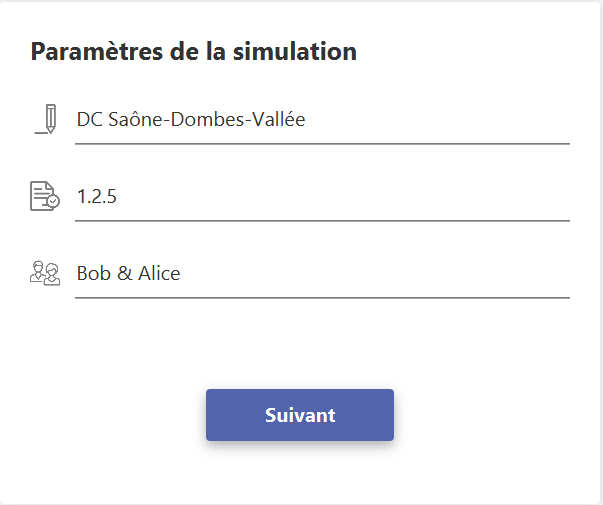
\includegraphics[height=6cm]{partie3/images/simulation.png}
		\caption{L'écran des paramètres de la simulation}
	\end{minipage}\hfill
	\begin{minipage}{0.48\textwidth}
		\centering
		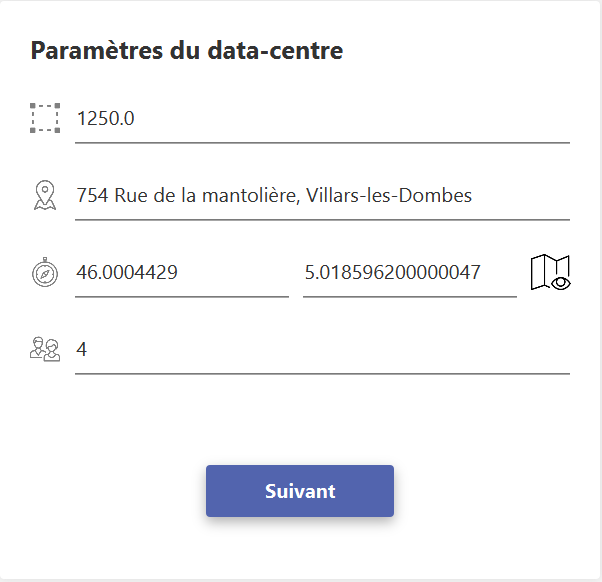
\includegraphics[height=6cm]{partie3/images/datacenter.png}
		\caption{L'écran des paramètres du centre de données}
	\end{minipage}\hfill
\end{figure}

\subsubsection{La géolocalisation}
Pour choisir l'adresse du centre de données, l'utilisateur a plusieurs choix. Il peut tout d'abord entrer une adresse qui sera automatiquement géocodée en coordonnées GPS. Il peut également entrer des coordonnées GPS qui seront automatiquement géocodées en une adresse. Il peut également choisir l'emplacement du centre de données en cliquant sur une carte.

\begin{figure}[h!]
	\begin{center}
		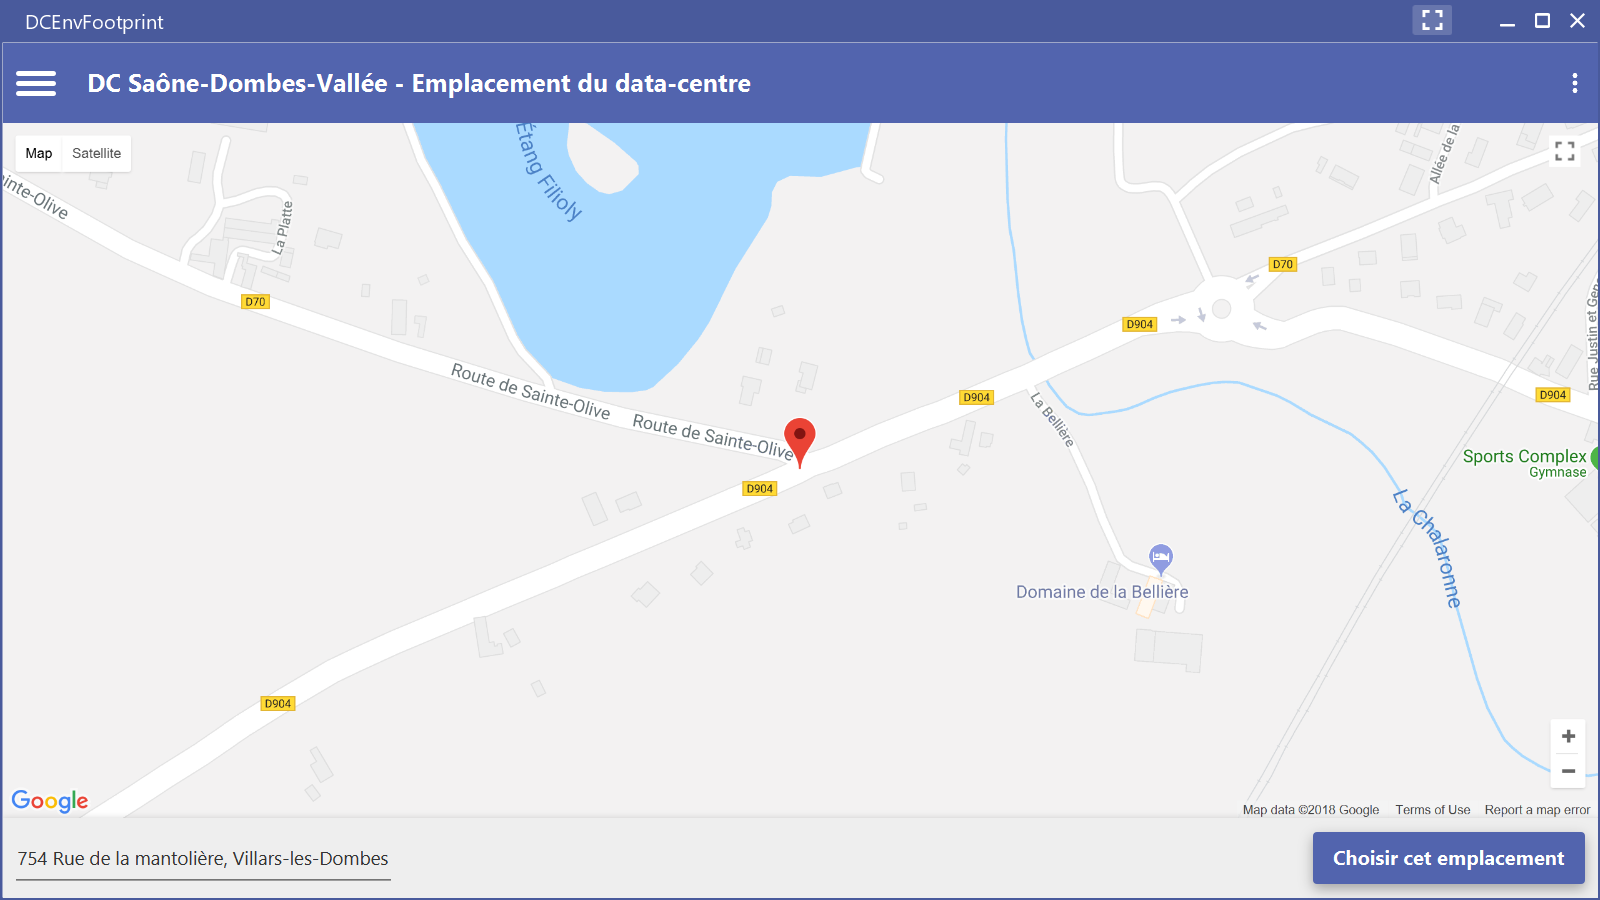
\includegraphics[scale=0.50]{partie3/images/carte.png}
		\caption{La carte permettant de choisir l'emplacement du centre de données}
	\end{center}
\end{figure}
\newpage
\subsubsection{La liste des périphériques de calcul}
L'utilisateur peut spécifier la liste des périphériques de calcul utilisés dans le centre de données. Une autocompletion depuis la base de données est fournie ce qui permet de choisir le bon modèle si il est disponible dans la base données. Une fois sélectionné la consommation d'énergie est automatiquement ajoutée.

\begin{figure}[h!]
	\begin{center}
		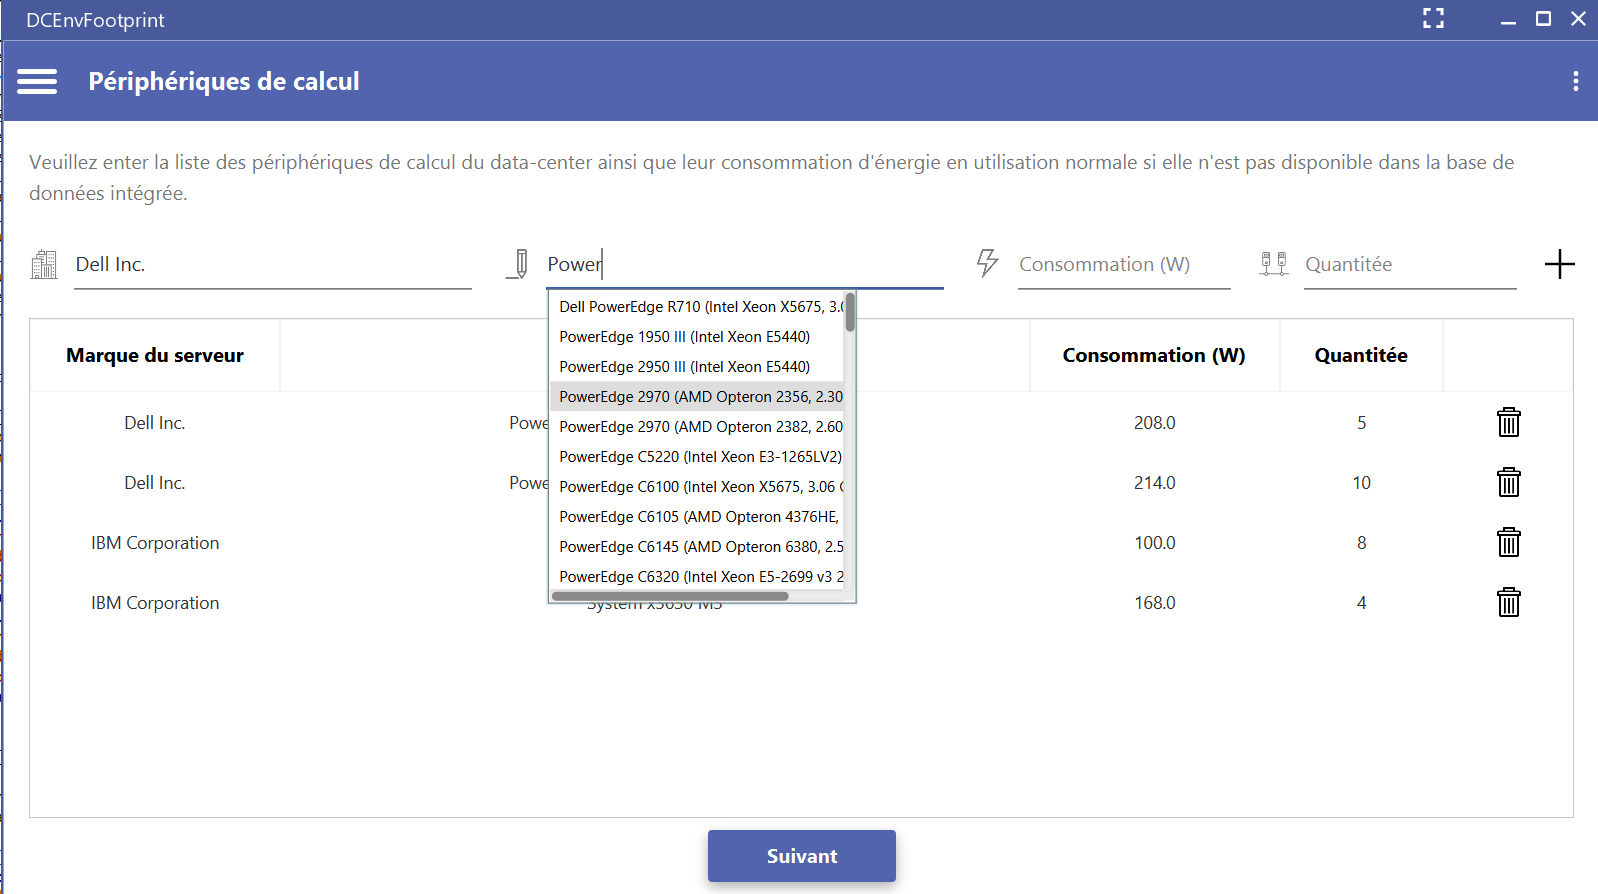
\includegraphics[scale=0.4]{partie3/images/calculation.png}
		\caption{L'écran permettant de saisir la liste des périphériques de calcul}
	\end{center}
\end{figure}

Il peut ensuite modifier n'importe quel modèle en cliquant sur les cellules du tableau. Il peut également supprimer un périphérique grâce au bouton sur la droite.

\subsubsection{La saisie des autres périphériques}
L'utilisateur peut également saisir les périphériques de stockage et les périphériques réseaux dans des écrans similaires à l'écran de saisie des périphériques de calcul. Cependant comme il n'existe pas de base de données pour ces équipements, il n'y a pas d'autocompletion. L'utilisateur devra se référer au manuel constructeur afin de définir la consommation d'énergie de son matériel.

\subsubsection{La gestion de la chaleur}
A partir des données entrées, le simulateur calcule automatiquement la dissipation de chaleur dans le centre de données. La méthode de calcul est basé sur un livre blanc de APC, une filière de Schneider Electric.\\
Pour répondre a cette quantité de chaleur, l'utilisateur peut choisir différentes formes de refroidissement dans la liste déroulante et les combiner. Comme certaines sources de refroidissement consomment de l'énergie, on laisse à l'utilisateur la possibilité de l'indiquer.

\begin{figure}[h!]
	\begin{center}
		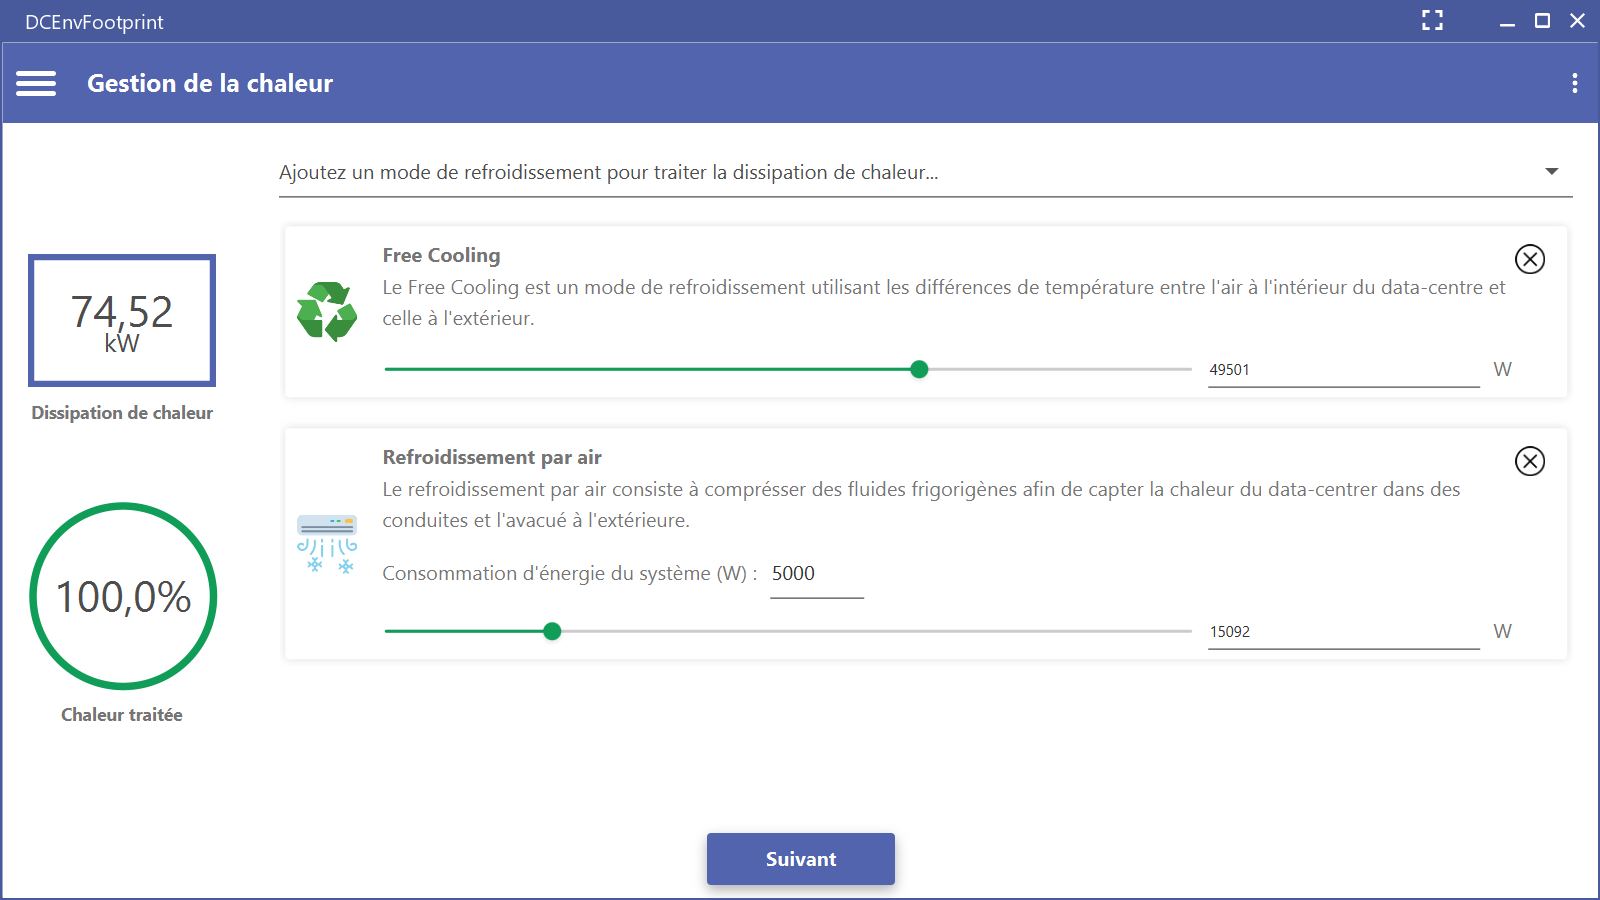
\includegraphics[scale=0.5]{partie3/images/chaleur.png}
		\caption{L'écran permettant de choisir les méthode de refroidissement}
	\end{center}
\end{figure}

\subsubsection{La réutilisation de chaleur}
Si le centre de données réutilise une partie de la chaleur créée par l'équipement informatique, l'utilisateur peut l'indiquer dans un écran dédié. Il peut également indiquer la quantité d'énergie utilisé pour ce retraitement de la chaleur. Cette information est importante car elle est prise en compte par certains indicateurs.

\subsubsection{La saisie des sources d'énergie}
Le simulateur calcule automatiquement la quantité d'électricité nécessaire au fonctionnement du centre de données. Il se base encore une fois sur un livre blanc d'APC.\\
Pour répondre à cette demande l'utilisateur peut ajouter des sources d'énergies depuis la liste déroulante et indiquer la quantité d'électricité qu'elle produit. Cet écran prend en compte l'énergie qui peut être produite sur site, comme vous pouvez le voir dans la capture d'écran suivante.

\begin{figure}[h!]
	\begin{center}
		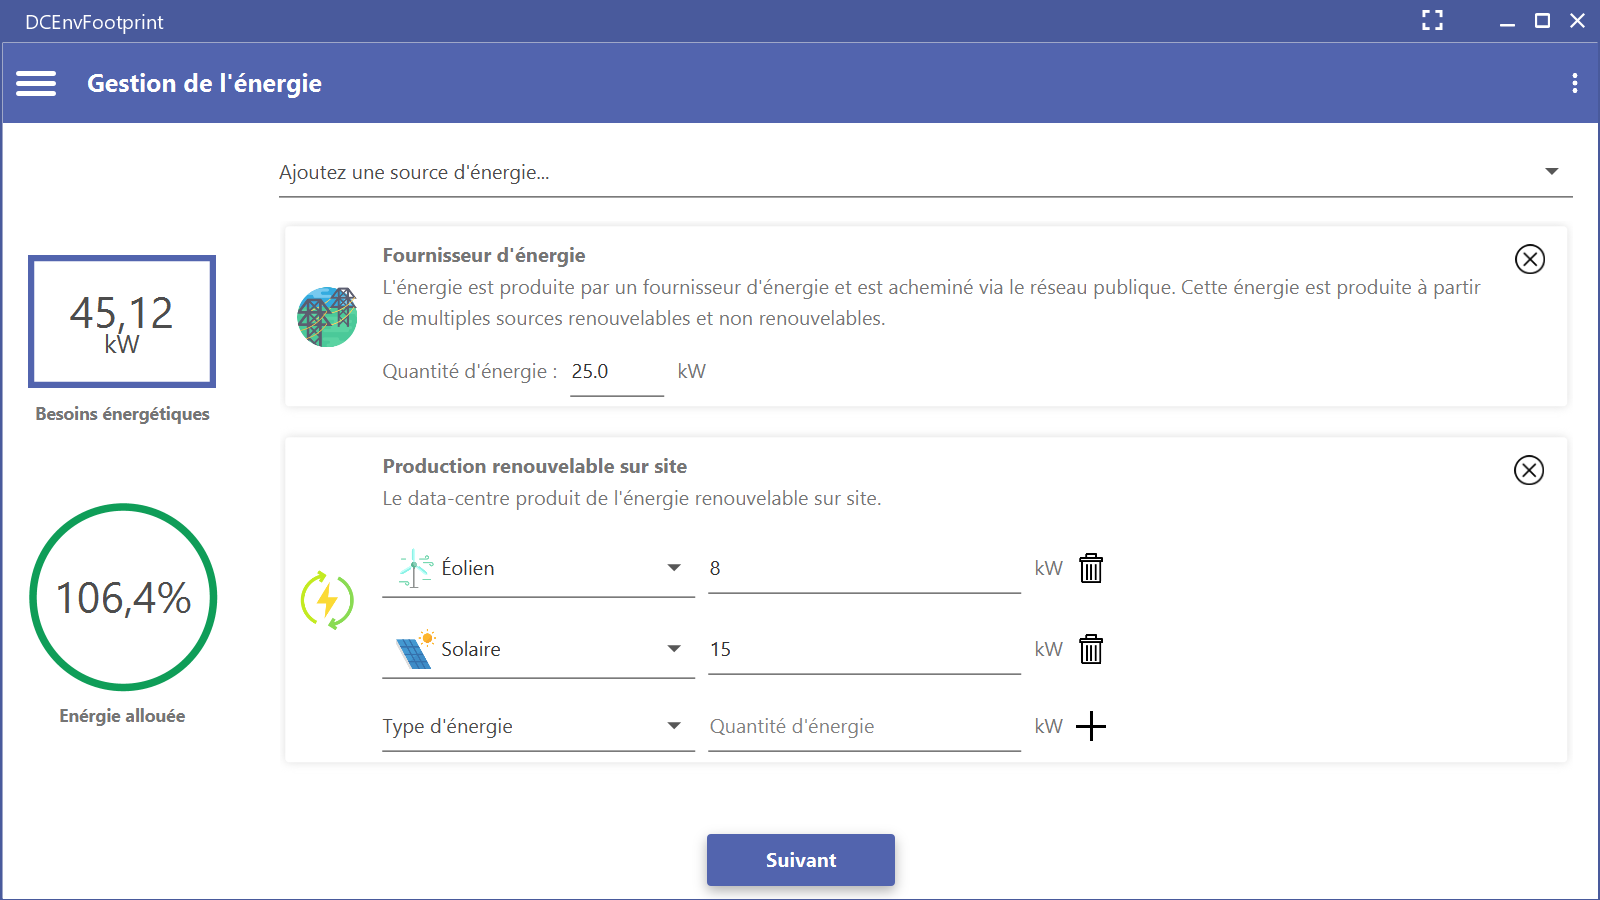
\includegraphics[scale=0.5]{partie3/images/energie.png}
		\caption{L'écran permettant de choisir les sources d'énergie}
	\end{center}
\end{figure}

\subsubsection{La vérification des champs}
Évidemment tous les champs modifiables par l'utilisateur sont vérifiés automatiquement et en temps réel afin qu'il ne mettent pas la simulation dans un état incohérent. L'utilisateur ne peut pas sauvegarder sa simulation ou passer à l'écran suivant si les champs contiennent des erreurs. Si il y a des erreurs lors de la sauvegarde, l'utilisateur est envoyé sur l'écran qui pose problème où les erreurs sont mis en évidences.

\begin{figure}[h!]
	\begin{center}
		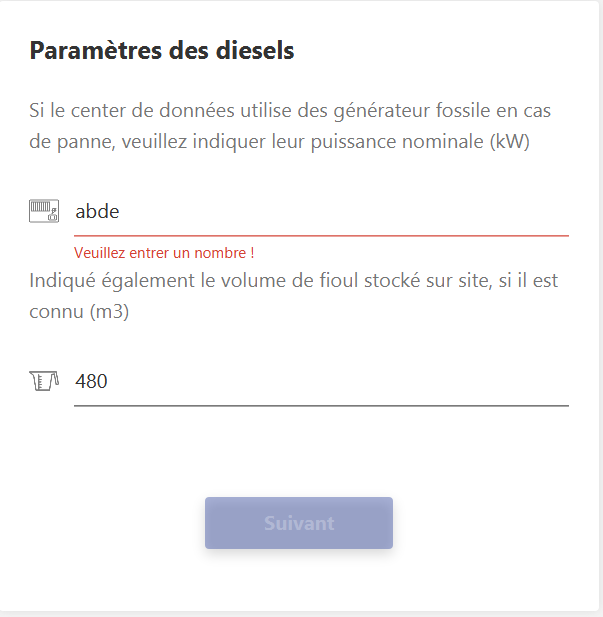
\includegraphics[scale=0.6]{partie3/images/verif.png}
		\caption{La gestion d'une erreur dans un champs}
	\end{center}
\end{figure}
\newpage
\subsubsection{La génération de rapport}
Une fois que l'utilisateur a entrer tous les paramètres dont le simulateur à besoin un rapport est généré automatiquement. Il calcule automatiquement les indicateurs et détaille le calcul de certains. Cependant il est loin d'être parfais, une  partie des indicateurs ne sont pas détaillés par faute de temps. Il aurait également été intéressant d'intégrer les sources systématiquement dans le raport. On remarque aussi que des commentaires utilisateurs ont été prévu, mais non implémentés.

Vous retrouverez en \hyperref[appendix:report]{Annexe C} un exemple de rapport généré par le simulateur.
\subsection{Le bilan des apprentissages}
Dans cette partie nous présenterons tous les apprentissages que ce stage m'a apporté. Nous commencerons tout d'abord par les apprentissages sur le plan technique et nous finirons par les informations que ce stage m'a donné sur le monde de la recherche.

\subsubsection{Les apprentissages technique}
Ce stage a tout d'abord permis d'améliorer mes compétences techniques sur le langage Java. J'ai pû mettre en œuvre les notions que m'a apporté la formation de l'IUT comme par exemple le modèle MVC, le modèle singleton, l'utilisation de git ou encore l'utilisation de JDBC pour la connexion aux base de données.\\

Même si je connaissais déjà via la formation donnée à l'IUT le langage SQL et PL/SQL je n'avais pas vraiment déjà essayé SQLite. J'en avais déjà beaucoup entendu parlé et avais vu de nombreux projets l'utiliser mais je n'avais jamais sauté le pas. L'utilisation de base de données dans le simulateur m'a donc permis de découvrir cette technologie qui s'avère très pratique.\\

Je me suis également beaucoup amélioré dans l'utilisation de JavaFX, en effet le simulateur comporte un interface graphique complexe qu'il n'a pas été évident de façonner. J'ai également pu découvrir la librairie JFoenix qui implémente le material design pour JavaFX que je réutiliserais à coup sûr dans des projets personnels.\\

Ensuite, je me suis auto-formé à une technologie pour la rédaction de documents internes et de ce rapport de stage : le langage \LaTeX. Il s'agit d'un langage de traitement de texte qui permet de rédiger des documents d'une grande qualité. Il est très utilisé dans le monde universitaire et de la recherche, je me suis donc dis que c'était l'occasion de le tester. J'ai beaucoup apprécié l'utiliser en comparaison à d'autres outils de traitement de texte comme Word, pour ne pas le citer, qui deviennent vraiment pénibles lors de la rédaction de documents exigeants. L'outils n'est pas forcément des plus simple à dompter, mais on s'habitue vite. De plus, comme il s'agit presque d'un langage de programmation, la méthodologie pour résoudre les problèmes est très similaire à celle utilisée lors de résolution de bugs. D'ailleurs, \LaTeX possède une communauté très active et une documentation extrêmement fournie (peut-être même trop) ce qui permet de trouver facilement les informations dont on a besoin.\\

Cependant, je remarque que la partie développement n'a pas été la partie la plus difficile à réaliser, j'avais déjà une bonne partie des connaissances nécessaires pour être efficace. Je n'ai donc pas été véritablement bloqué sur des problèmes techniques, mais plus sur des problèmes d'ergonomie ou de maquettage.

\subsubsection{La découverte du Green IT}
Ce stage m'a permis de découvrir concrètement ce qu'est le Green IT. J'ai eu la chance de travailler dans ce laboratoire qui est reconnu internationalement pour ces apports dans ce domaine. Cela m'a beaucoup intéressé, car comme je l'ai déjà précisé je suis depuis tout petit passionné des problématiques environnementale et espère pouvoir les intégrer dans mon projet professionnel dans le futur. La recherche bibliographique que j'ai réaliser m'a beaucoup apporté, j'ai pu mieux comprendre les enjeux de chacun des acteurs et comprendre en quoi ce domaine va devenir de plus en plus important avec le temps.\\

Je suis d'ailleurs désormais des sites web d'actualités sur le Green IT ainsi qu'un groupe Linkedin, ce qui me permet de faire un petit peu de veille technologique sur ces problématiques.

\subsubsection{La découverte du milieu de la recherche}
Grâce à ce stage j'ai pu en découvrir un petit peu plus sur le milieu de la recherche en informatique. J'ai découvert la très forte institutionnalisation des structures qui s'entremêlent les unes dans les autres dès la rédaction de mon modèle de convention de stage, étant en effet sous contrat avec le CNRS de Grenoble pour travailler dans le Laboratoire de l'Informatique du Parallélisme dans le bâtiment de l'ENS Lyon.\\

J'ai remarqué la grande part de rédaction que prédispose le travail dans ce milieu : thèses, publications scientifiques, rapport d'activité etc. le travail est systématiquement valoriser par un document. Si l'on n'aime pas rédiger il est évident que travailler dans ce milieu risque d'être difficile, mais je suppose que l'aisance vient avec les temps et que les doctorants qui sortent de thèse sont déjà beaucoup plus à l'aise en rédaction qu'une étudiant en fin de deuxième année de DUT Informatique.\\

J'ai cependant été un petit peu surpris de remarquer le manque de travail en équipe. Je m'imaginais au contraire de très grandes équipes travaillant ensemble sur un même sujet, mais il semblerait plutôt que chacun travaille de son coté avant de le compiler avec ces collègue. Je garde cependant à l'esprit que la vision que j'ai eu durant ce stage n'est peut-être pas représentatif de toutes les équipes de recherches de tous les laboratoires, et que cette situation est peut-être conjoncturelle.\\

Cependant cela n'a pas ébranler mon souhait d'orienter un petit peu plus mon projet professionnel vers la recherche. Je le confirme d'ailleurs avec mon choix de rejoindre un le département de recherche et développement de l'entreprise qui m'accueillera dans le cadre de mes 3 ans d'alternance à l'INSA Lyon à partir de Septembre prochain.
\subsection{Bilan humain du stage}
L'environement humain durant ce stage était évidemment un petit peut particulier. Tout d'abord j'étais seul sur le projet. D'un côté c'est très appréciable car on a une liberté de mouvement et une autonomie gigantesque, mais j'aurais beaucoup apprécié travailler avec quelqu'un d'autre. Même si les autres membres de l'équipes étaient présent si j'avais une question et que j'étais en compagnie de mon camarade Lucas, j'ai ressenti une certaine solitude dans le travail.\\

Pour résumer une seule phrase l'ambiance au sein de l'équipe je dirais que les membres de l'équipes sont tous extrêmement sympathiques, mais également extrêmement occupés. En effet, les doctorant sont en plein phase de rédaction de thèse, les universitaires permanents comme Laurent Lefèvre, mon maître de stage sont souvent en déplacement pour d'autres projets ou pour des obligations institutionnelles, enfin les ingénieurs quant-à-eux sont sous le feu des pannes en cours.\\

Même si je comprends tout à fait les problèmes d'ordre organisationnel que cela prédispose, j'ai également regretté qu'il n'y ait pas eu plus de groupes de travail, cela aurait permis de connaitre un petit plus les membres de l'équipe que je ne croise pas tous les jours et de me rendre compte du travail de chacun, souvent complexe.\\

Malgré cela l'ambiance au sein de l'équipe étais très bonne et les pause de midi nous permettaient quand même d'échanger entre nous.
\newpage
\section*{Conclusion}
\addcontentsline{toc}{section}{Conclusion}


\newpage
\addcontentsline{toc}{section}{Glossaire}
\printglossaries
\newpage
\addcontentsline{toc}{section}{Table des figures}
\listoffigures
\addcontentsline{toc}{section}{Liste des tableaux}
\listoftables

\newpage
\addcontentsline{toc}{section}{Sources}
\bibliographystyle{plain}
\bibliography{sources}

\newpage
\part*{Annexes}
\addcontentsline{toc}{section}{Annexes}
\appendix

\startcontents[annexes]
\printcontents[annexes]{ }{1}{}
\newpage
\part*{Annexe A}
\section{Calcul du KPI Energy Consumption ($KPI_{EC}$)}
\label{appendix:kpiec}
Le $KPI_{EC}$ est définie par la formule suivante que nous allons détailler :
\[KPI_{EC} = EC_{SP} + EC_{FEN} + EC_{REN} + (EC_{TH} \times K_{TH})\]

\subsection{Consommation électrique du réseau ($EC_{SP}$)}
Il s'agit de la quantité d'énergie obtenue depuis le réseau électrique et qui est relevée sur les compteurs du fournisseur d'énergie.
Cette valeur prend également en compte l'énergie issue d'une boucle interne de distribution d'électricité et les pertes dans les transformateurs.

\subsection{Consommation électrique d'énergie fossile ($EC_{FEN}$)}
Il s'agit de la quantité d'énergie produite localement à partir de sources d'énergie fossile, comme par exemple des groupes électrogènes. Elle est mesurée à la sortie de la source d'énergie si elle est dédiée au data-centre ou à l'entrée de ce dernier si la source est partagée avec d'autres sites.

\subsection{Consommation électrique d'énergies renouvelables ($EC_{REN}$)}
Il s'agit de la quantité d'énergie produite localement à partir de sources renouvelables. Le mode de mesure est le même que pour l'$EC_{FEN}$.

\subsection{Consommation d'énergie thermique ($EC_{TH}$)}
Il s'agit de la quantité d'énergie thermique livrée, quelle soit chaude ou froide. On la mesure à l'entrée du data-centre via un compteur de calories.

\subsection{Facteur de conversion d'énergie thermique ver électrique ($K_{TH}$)}
Il s'agit du facteur de conversion s'il est connu et certifié, si ce n'est pas le cas on utilisera la valeur par défaut $0,43$ qui correspond à une installation de référence.
\newpage
\part*{Annexe B}
\section{Calcul de l'énergie perdue dans les lignes HTA}
\label{appendix:aclosses}
\subsection{L'effet de peau}
L'effet de peau est un phénomène électromagnétique faisant qu'a haute fréquence, le courant est transmis dans la section du conducteur la plus proche de la surface. La densité du courant décroît exponentiellement à mesure que l'on s'éloigne de la périphérie du conducteur ce qui entraine une augmentation de la résistance de ce dernier et donc des pertes d'énergie.\\

La quantité d'énergie perdu est définie par la formule suivante :

\[P_{peau}=(1 - exp(\frac{-dR_l}{Lc})) \times P_{nominale} \]

\begin{center}
	\begin{tabular}{|c|c|}
		\hline 
		Paramètre & Définition et unité \\
		\hline
		$P_{peau}$ & Énergie perdue par effet de peau \\ 
		& (kW) \\
		\hline
		$d$ & Longueur du câble \\
		& (m) \\	
		\hline	
		$R_l$ & Résistivité du câble \\
		& (\SI[per-mode = symbol]{}{\ohm\per\m}) \\
		\hline
		$L$ & Inductance par mètre \\
		& (\SI[per-mode = symbol]{}{\henry\per\m}) \\
		\hline
		$c$ & Célérité de la lumière dans le vide \\ 
		& (\SI[per-mode = symbol]{3e8}{\m\per\s}) \\
		\hline
		$P_{nominale}$ & La puissance nominale de la ligne \\ 
		& (kW) \\
		\hline
	\end{tabular}
\end{center}

\subsubsection{La résistivité du câble}
La résistivité du câble représente sa capacité à s'opposer à la circulation du courant électrique. Cela correspond à la résistance d'un tronçon du matériaux conducteur du câble d'un mètre de longueur et d'un mètre carré de section \cite{Resistivite}.\\

Elle est définie par la formule suivante :

\[R_l=\frac{I_B}{2\pi a \sigma \delta}\]

\begin{center}
	\begin{tabular}{|c|c|}
		\hline 
		Paramètre & Définition et unité \\
		\hline
		$R_l$ & Résistance par unité de longueur \\
		& (\SI[per-mode = symbol]{}{\ohm\per\m}) \\
		\hline
		$I_B$ & Coefficient de correction de Bessel \\
		& (1,1) \\
		\hline
		$a$ & Rayon du câble \\
		& (\SI{}{\m}) \\
		\hline
		$\sigma$ & Conductivité du métal \\
		& (\SI[per-mode = symbol]{}{\siemens\per\m}) \\
		\hline
		$\delta$ & Épaisseur de peau du câble \\
		& (m) \\	
		\hline
	\end{tabular}
\end{center}

\subsubsection{L'épaisseur de peau du câble}
L'épaisseur de peau du câble détermine la largeur de la zone où se concentre le courant dans le câble.

Elle est définie par la formule suivante :

\[\delta=\frac{1}{\sqrt{\pi f \mu_0\sigma}}\]

\begin{center}
	\begin{tabular}{|c|c|}
		\hline 
		Paramètre & Définition et unité \\
		\hline
		$\delta$ & Épaisseur de peau du câble \\
		& (m) \\
		\hline
		$f$ & Fréquence du courant \\
		& (\SI{}{\hertz}) \\
		\hline
		$\mu_0$ & Perméabilité magnétique du vide \\ 
		& (\SI[per-mode = symbol]{4\pi e-7}{\henry\per\m}) \\
		\hline
		$\sigma$ & Conductivité du métal \\
		& (\SI[per-mode = symbol]{}{\siemens\per\m}) \\
		\hline
	\end{tabular}
\end{center}

\subsubsection{L'inductance par unité de longueur}
L'inductance est la quantification de l'énergie électromagnétique qui apparait lorsque le courant parcourt le câble.\\

Elle est définie par la formule suivante :

\[L=\frac{\pi}{\mu}\ln(\frac{d}{a})\]

\begin{center}
	\begin{tabular}{|c|c|}
		\hline 
		Paramètre & Définition et unité \\
		\hline
		$L$ & Inductance par mètre \\
		& (\SI[per-mode = symbol]{}{\henry\per\m}) \\
		\hline
		$\mu$ & Perméabilité magnétique ambiant ($\approx \mu_0$) \\
		& (\SI[per-mode = symbol]{}{\henry\per\m}) \\
		\hline
		$d$ & Espace entre deux lignes (\emph{A vérifier}) \\ 
		& (\SI{}{\m}) \\
		\hline
		$a$ & Rayon du câble \\
		& (\SI{}{\m}) \\
		\hline
	\end{tabular}
\end{center}

\subsection{L'effet corona}
L'effet corona est dû à l'ionisation des molécules d'air le long des lignes électriques. Une partie de l'énergie est dissipée dans l'air. Cet effet varie selon les conditions métrologiques.\\

La quantité d'énergie perdu par effet corona est définie par la formule suivante :

\[P_{corona}=\frac{k_0}{k_d}(f + 25)\sqrt{\frac{a}{d}}[V_0 - g_0k_iak_d\ln(\frac{d}{a})]^2 \times 10^{-5} \times l\]

\begin{center}
	\begin{tabular}{|c|c|}
		\hline 
		Paramètre & Définition et unité \\
		\hline
		$k_0$ & Constante \\
		& (241) \\
		\hline
		$k_d$ & Densité de l'air \\
		& (\SI[per-mode = symbol]{}{\hecto\pascal}) \\
		\hline
		$f$ & Fréquence \\ 
		& (\SI{}{\hertz}) \\
		\hline
		$a$ & Rayon du câble \\
		& (\SI{}{\cm}) \\
		\hline
		$d$ & Espace entre deux lignes (\emph{A vérifier}) \\
		& (\SI{}{\cm}) \\
		\hline
		$V_0$ & Tension phase neutre \\
		& ($Tension\ ligne\ ligne/1.73\ \SI{}{\kilo\volt}$) \\
		\hline
		$g_0$ & Rigidité diélectrique de l'air \\
		& (\SI[per-mode = symbol]{21}{\kilo\volt\per\cm}) \\
		\hline
		$k_i$ & Facteur de correction du câble \\
		& (\emph{Se référer aux tables constructeur}) \\
		\hline
		$l$ & Longueur du câble \\
		& (km) \\
		\hline
	\end{tabular}
\end{center}
\stopcontents[annexes]
\resumecontents

\newpage
\thispagestyle{empty}
\begin{spacing}{1}
	\newgeometry{left=2cm,right=2cm,top=1cm,bottom=1cm} %Marges centrées de la page de garde
	
	\newcommand{\HRule}{\rule{\linewidth}{0.5mm}}
	\begin{center}
		\textsc{\LARGE Rapport de stage - 2\up{eme} année \\ DUT Informatique}\\
		\HRule \\[0.8cm]
		{ \huge \bfseries Simuler l'empreinte environnementale des centres de données}\\[0.4cm]
		\HRule \\[0.5cm]
		
		\textsc{\Large Bastien Marsaud}\\
		\textsc{\Large 9 Avril - 15 Juin 2018}\\
	\end{center}
	
	\section*{Résumé}
	Étudiant en deuxième année de DUT informatique à l'IUT Lyon 1, j'ai effectué mon stage de fin de cursus au Laboratoire de l'Informatique du Parallélisme à l'ENS Lyon. Très intéressé par le milieu de la recherche et par les problématiques environnementale j'ai initié la conception d'un simulateur d'empreinte environnementale des centres de données. Ce simulateur permettra à terme d'aider les urbanistes et le architectes dans la conception et l'intégration des centre de données sur le territoire. Il sera capable à partir d'une multitude de données entrées par l'utilisateur de générer automatiquement un rapport complet présentant les caractéristiques du centre de données ainsi que ses scores pour les différents indicateurs réputés du domaine.\\
	Dans ce rapport de stage vous découvrirez le Laboratoire de l'Informatique du Parallélisme en tant qu'organisation, les différentes étapes du projet de la phase de découverte du sujet et de conception d'une bibliographie à la phase de développement, mais également mon ressenti sur cette expérience dans le monde de la recherche et ce que j'ai découvert techniquement et humainement.\\\\
	
	\textbf{Mots clefs :} informatique, green IT, datacenter, recherche, environement, énergie, simulation, économie, urbanisme

	\begin{figure}[b]
		\begin{minipage}[c]{.48\linewidth}
			\center
			
\includegraphics[width=5cm]{pagedegarde/images/logo_iut.png}
		\end{minipage} \hfill
		\begin{minipage}[c]{.48\linewidth}
			\center
			
\includegraphics[width=4cm]{pagedegarde/images/logo_lip.png}
		\end{minipage}
	\end{figure}
\end{spacing}

\end{document}